\documentclass{tesisITAM}
\usepackage[utf8]{inputenc}
\usepackage{fontspec}

\setromanfont[
BoldFont=timesbd.ttf,
ItalicFont=timesi.ttf,
BoldItalicFont=timesbi.ttf,
]{times.ttf}
% Arial
\setsansfont[
BoldFont=arialbd.ttf,
ItalicFont=ariali.ttf,
BoldItalicFont=arialbi.ttf
]{arial.ttf}
% Courier New
\setmonofont[Scale=0.90,
BoldFont=courbd.ttf,
ItalicFont=couri.ttf,
BoldItalicFont=courbi.ttf
]{cour.ttf}

\usepackage[backend=bibtex,style=numeric-comp,natbib=true,sortcites=true,block=space,sorting=none]{biblatex}
\addbibresource{efinfo}


\usepackage[font=scriptsize,labelfont=bf]{caption}



\title{Proyecto: Biblioteca de Arte Mexicano}

\year{2015}



\begin{document}

	\pagenumbering{gobble}
	\maketitle
	\publicationrights

	\selectlanguage{spanish}
	\setcounter{page}{1}
	\pagenumbering{roman}

	\tableofcontents
	\listoffigures
	\listoftables
	\newpage

	\pagenumbering{arabic}
	\setcounter{page}{1}

	%%%%%%%%%%%%%%%%%%%%%%%%%%%%%%%%%%%%%%%%%%%%%%
	% CONTENT
	%%%%%%%%%%%%%%%%%%%%%%%%%%%%%%%%%%%%%%%%%%%%%%

	\chapter{Introducción}
\label{ch:intro}


\section{Antecedentes}

Este trabajo se realizó como parte del Programa de Estímulos a la Investigación de CONACYT y la empresa   OCRMX. 

La empresa OCRMX S.A. de C.V. se dedica al negocio de digitalización masiva de documentos  pertenecientes a múltiples dominios.
Actualmente desea desarrollar un sistema completo de control de documentos y registros que sean funcionales para generar oficinas “sin papel” en los procesos relacionados con la administración empresarial de recursos humanos. Estos procesos generan documentos como: Contratos, registros de capacitación, fichas del personal, registros de baja, documentación sobre pagos de nómina, documentación sobre seguridad social, entre otros. La colección de este tipo de documentos se denomina: Expediente. La administración del expediente consta de varias fases tales como:
\begin{itemize}
 
\item	Digitalización de documentos, para poder administrar mediante el nuevo sistema las versiones históricas  (archivo muerto) de los expedientes.
\item	Generación de documentos (ya en el sistema, sin papel).
\item	Configuración y administración del modelo de contenido de los documentos: En esta fase es necesario que se designen los campos y componentes (fotografías, firmas, impresiones digitales, etc.) de cada documento, así como el ciclo de revisiones y aprobaciones al cual se debe someter según roles determinados de usuarios.
\end{itemize}

OCRMX busca  desarrollar un sistema de administración de contenidos (CMS) o adaptar uno abierto que le  permita tener tres sistemas principales 
\begin{enumerate}

\item 	\textbf{Colección de contenidos}:tiene por finalidad administrar la publicación y almacenamiento de la información recibida "cruda" convirtiéndola de información no estructurada a estructurada.  Este sistema debe permitir la autoría (creación de nuevos documentos), la adquisición de documentos (recolectar contenido de otras fuentes existentes), extracción de información relevante y edición de contenido. 
\item 	\textbf{Administración de sistema y contenidos}: En el cual se almacenan los componentes. Contiene el repositorio, las interfases de administración, el flujo de trabajo  y las conexiones entre sistemas.
\item 	\textbf{Publicación de contenidos}: Que obtiene componentes del sistema de almacenamiento y los convierte en publicaciones.
\end{enumerate}


La empresa OCRMX también busca aprovechar la información de sus usuarios que le permita: 
\begin{itemize}

\item Detalles sobre el contenido: tipos de componentes, en qué etapa del ciclo de vida se encuentran, etc.
\item El nivel uso del sistema y los contenidos que genera o revisa el personal, para detectar cuellos de botella o necesidades de capacitación.
\item Qué contenido  se utiliza en publicaciones y qué contenido puede ser destruido.
\item 	Quién utiliza qué contenido y quién ha contribuido en cada documento.
\end{itemize}

Además el sistema de publicación es el encargado de extraer el contenido del repositorio y crear de forma automatizada publicaciones con dicho contenido.

	Sus componentes y procesos principales son:
	\begin{itemize}
    \item 	Plantillas de publicación: Los cuales son programas que construyen publicaciones de manera automática.
    \item 	Servicios de publicación: Herramientas que controlan qué y cómo es publicado un contenido.
    \item 	Conexiones: Herramientas y métodos que se utilizan para incluir datos desde otros sistemas y publicaciones externas.
    \item 	Publicaciones en línea.
    \item 	Publicaciones genéricas: documentos electrónicos o impresiones.
    \end{itemize}



\section{Datos}
La empresa OCRMX necesita administrar la información de una colección de arte mexicano que  consta de aproximadamente  3,500 documentos que contienen imágenes y  texto. OCRMX necesita  adaptar un sistema para manejar esta colección. El manejador que eligieron fue \href{http://dspace.org}{DSapce} y la unidad de análisis es una página. 
Para este proyecto se contrataron dos equipos, uno de la  Universidad Nacional Autónoma de México (UNAM) y otro del Instituto Tecnológico Autónomo de México (ITAM).

\section{Objetivo}
El proyecto “Biblioteca de Arte Mexicano” busca que los usuarios puedan explorar de una manera fácil e intuitiva la historia del arte mexicano. Para lograrlo se proponen la generación de algoritmos para resumir contenido, extraer entidades y sus relaciones, análisis de tópicos en periodos determinados y relación de las obras por contenido. 
Esperamos este proyecto contribuya  a la generación de conocimiento en áreas de alta tecnología de recursos humanos pertenecientes al programa de Maestría en Ciencia de Datos del Instituto Tecnológico Autónomo de México (ITAM).

\section{Producto}
Con las actividades descritas a continuación  el equipo del ITAM desarrolló un proceso para extraer similitudes entre documentos. Este producto se compone de tres subprocesos: procesamiento de texto, procesamiento de imágenes y  procesamiento de clickstream. Cabe destacar que el producto desarrollado es todo un proceso y  no solamente algoritmos.   

Con el fin de obtener un producto completo en lugar de una colección de scripts, se optó por agrupar los algoritmos en un paquete \texttt{itm} (ITAM Text Miner). De este modo la instalación es relativamente sencilla y revisa las dependencias de \texttt{Python} automáticamente. Además esto  permite guardar ejecutables en el \texttt{PATH} del servidor, lo que permite correr los códigos desde cualquier ruta.



\section{Entregables}

Respondiendo a las necesidades de la empresa OCRMX el ITAM se comprometió a realizar los siguientes entregables: 
\begin{enumerate}
\item Definición de tecnologías, infraestructura básica y arquitectura. Definición del pipeline completo del proyecto. 
\item Integración de los datos disponibles, documentación de la metodología y procesos empleados. Generación de estándares, metodologías y ETLs para la inserción de nuevos documentos.
\item Documentación del listado de algoritmos, criterio de selección de éstos, entrenamiento y validación de los prototipos. \item Implementación (en conjuntos de entrenamiento y prueba), automatización y medidas de desempeño. Prototipos de presentación de resultados.
\item Presentación del desempeño de resultados obtenidos con los modelos finales. Visualización de estos en formato digital. 
Despliegue, automatización de procesos faltantes y documentación final.

\end{enumerate}

Para ello se realizaron las siguientes actividades: 

\begin{itemize}

\item Adquisición del estado de los datos y metadatos con los que cuenta OCRMX en la biblioteca de Arte Mexicano.
\item	Recolección bibliográfica, artículos académicos y de la industria para establecer el estado del arte.
\item	Adquisición de conocimiento de arquitectura de datos, tecnología y de sistemas que actualmente posee OCRMX.
\item 	Estructura de los datos que actualmente posee OCRMX, así como de los procesos que tienen para generarlos de manera continua (formatos, flujos, tablas, motores, drivers, periodicidad, tamaño actual, crecimiento, etc.)
\item 	Solicitud de datos  y recepción de los mismos.
\item 	Establecimiento de arquitectura del equipo de Ciencia de Datos (DS). Construcción y montado en Amazon AWS. Conexiones y accesos. Establecimiento de niveles de seguridad.
\item 	ETL (scripts  de extracción, transformación y carga) de datos proporcionados por OCRMX a la arquitectura de DS.
\item 	Listado de algoritmos a implementar.
\item 	Implementación de algoritmos. 
\item 	Visualización y métricas de resultados.
\item 	Establecimiento de proceso continuo.
\item 	Sugerencias de implementación.
\item 	Elaboración de reporte técnico

\end{itemize}



\section{Flujo del proyecto}
\subsection{Arquitectura}
Para las primeras pruebas del  proyecto “Desarrollo de un Sistema de Publicación de Biblioteca de Arte Mexicano” se eligió la nube de Amazon para almacenar y procesar los 890 Gb de información.  Para tomar esta decisión se compararon los precios de almacenamiento y de procesamiento por el tipo de máquinas que ofrece Amazon (AWS) y Google. Lo anterior considerando que ambos servicios ofrecen los servicios necesarios para el procesamiento que se requieren para el proyecto.

En general las características de los servicios de almacenamiento y procesamiento son muy similares en ambas empresas, el precio cambia cuando se trata de procesamiento en computadoras más complejas. Por ejemplo, en el caso de una máquina en AWS de 8 cores y 64 GB de memoria, el precio por hora es de 7 centavos de dólar por hora. Si se compara contra la máquina más similar de Google, una máquina de 16 cores con 60 GB de memoria, el precio es muy similar en centavos de dólar por hora.

Con base en lo anterior y considerando que podemos controlar las horas de procesamiento, se consideró que el precio entre ambos servicios no es un factor decisivo. Sin embargo, nuestra experiencia con los servicios que ofrece Amazon es más extensa que con los de Google. Con base en esto y dado que las diferencias de precios no son significativas para fines de procesamiento y almacenamiento, se decidió utilizar los servicios de Amazon Web Service (AWS).

Para la realización de las pruebas se utilizaron los leguajes de  Python, Bash y R. Una vez definido los procesos  e integrado las ideas del equipo del GIL (UNAM) se decidió solamente usar Python para la realización del proyecto y procesar todo en los servidores de la empresa OCRMX.   

\subsection{Listado de Algoritmos}

Los algoritmos que componen el proceso desarrollado por el ITAM son los siguientes:



\textbf{Procesamiento de Texto}

\begin{itemize}
\itemsep1pt\parskip0pt\parsep0pt
\item
  Term frequency – Inverse document frequency (TF-IDF)
\item
  Latent Dirichlet allocation (LDA)
\end{itemize}

\textbf{Procesamiento de Imagen}

\begin{itemize}
\itemsep1pt\parskip0pt\parsep0pt
\item
  Filtro de extracción de imágenes
\item
  Reducción de imágenes
\item
  Singular Value Decomposition (SVD) \& K-Means
\item
  Local Sensitive Hashing (LSH)
\end{itemize}

\textbf{Procesamiento de Clickstream}
\begin{itemize}
\item Estructurar
\item Sesionizar
\item Enriquecer 
\end{itemize}

	\chapter{Producto}
\label{producto}


\section{Orquestación}

Un sistema de análisis a gran escala necesita coordinar y gestionar de manera robusta y confiable los procesos del flujo de trabajo, a esto se le llama orquestación. Existen varios orquestadores, tales como \texttt{Oozie, Azkaban y Luigi}. Para este proyecto se eligió  \href{http://luigi.readthedocs.org/en/stable/}{\texttt{luigi}}, que fue desarrollado por Spotify en el lenguaje \texttt{Python}. Este esquema tiene varias ventajas sobre los scripts simples, algunas de las cuales se enumeran a continuación:

\begin{enumerate}
\item \textbf{Modularidad}: El código se segmenta en pasos definidos, lo que facilita su mantenimiento y expansión.
\item \textbf{Robustez}: Se requiere que todos los pasos serializen sus resultados a disco, lo que hace que el sistema sea resistente a fallas y que no tenga que repetir todo el proceso después de un error.
\item \textbf{Idempotencia}: Si se programa correctamente, los procesos sólo corren una vez. Incluso si se corre el proceso una segunda vez, sólo corre lo que no haya sido corrido antes.
\item \textbf{Paralelismo}: Es bastante sencillo paralelizar los procesos que convenga para utilizar los núcleos de un servidor grande de manera eficiente.
\end{enumerate}



 \texttt{Luigi} ofrece estas ventajas, lo único que se requiere es que los pasos tengan entradas y salidas bien definidas; un proceso únicamente requiere sus dependencias para correr y debe arrojar los resultados que necesite la siguiente sección.

\texttt{Luigi} corre nativamente en \texttt{Python}, por lo que se puede hacer cualquier cosa que se pueda hacer en \texttt{Python}. Esto incluye llamar códigos en \texttt{shell}, \texttt{R} y muchos otros lenguajes. La mayoría de los procesos se hicieron directamente en \texttt{Python} por simplicidad, pero algunos se dejaron en otros lenguajes por su facilidad de uso.

A continuación se describe a grandes rasgos los pasos que componen el  \emph{pipeline} o diagrama de flujo. Cabe mencionar que esta es una descripción didáctica del proceso. Internamente hay algunos procesos que se efectúan en un orden ligeramente distinto al aquí presentado, por cuestiones computacionales.

 A continuación se muestra el diagrama de flujo de todo el proyecto, representado en la figura \ref{flujo}, las partes en verde son las correspondientes a los algoritmos  del ITAM, las figuras en blanco son los procesos desarrollados por el equipo de la UNAM/GIL.

\begin{figure}[H]
\centering
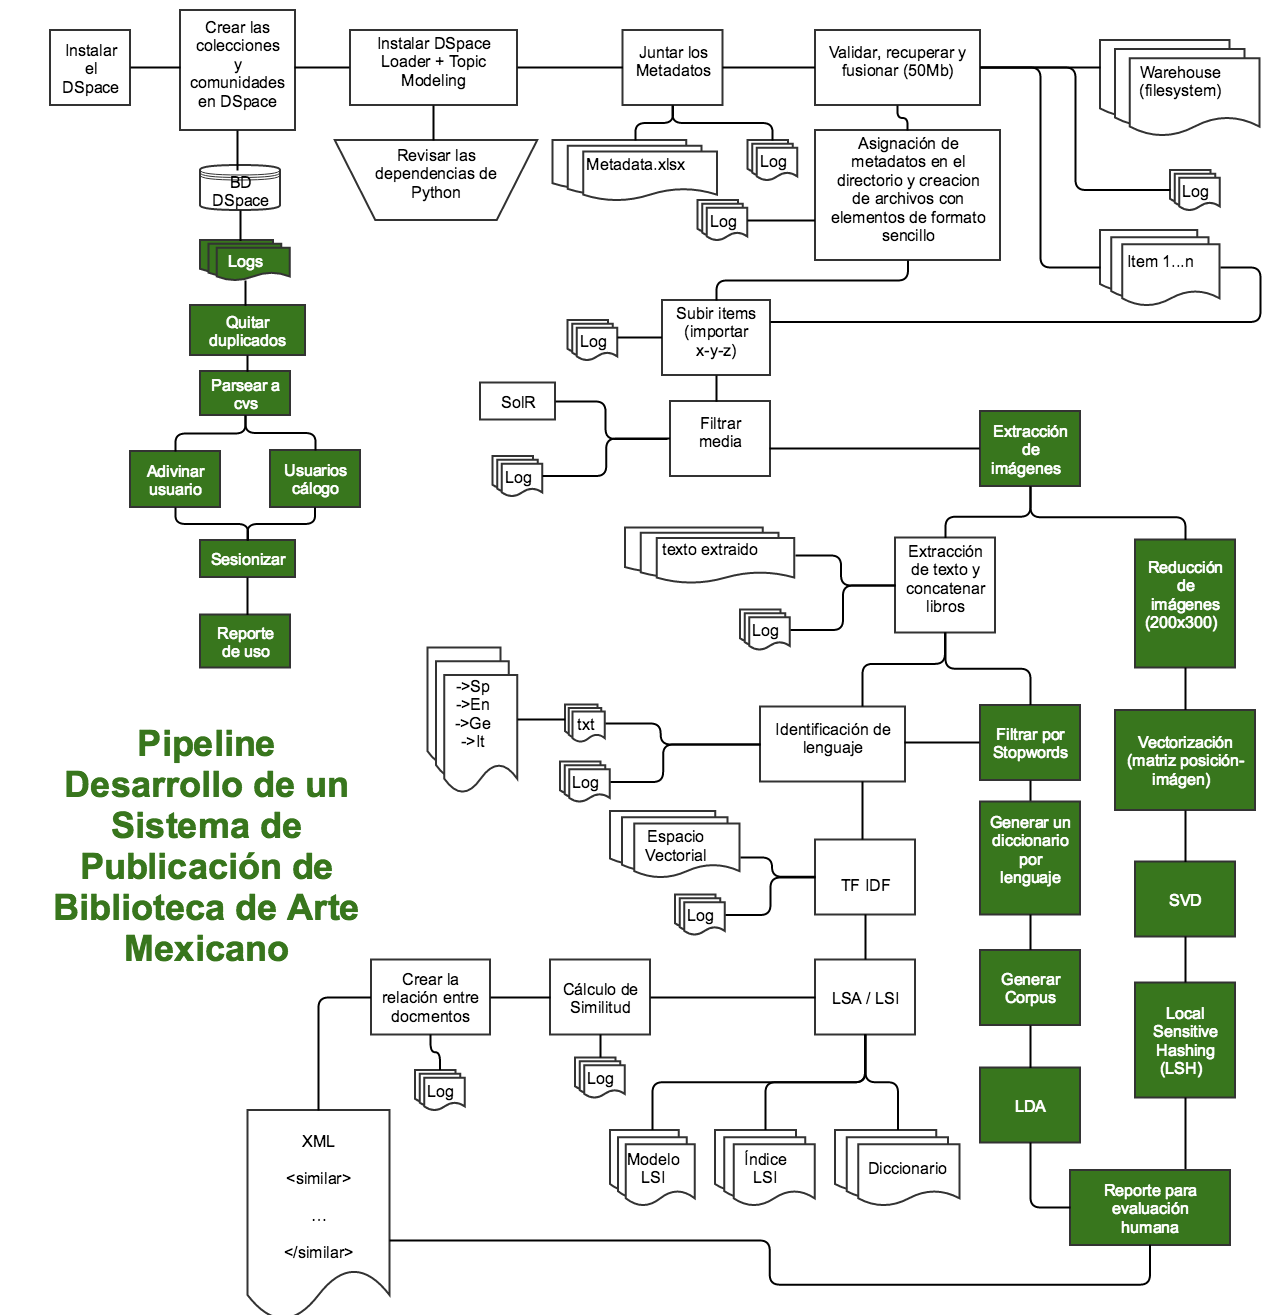
\includegraphics[width=1\textwidth]{Figures/pipeline.png}
\caption{Diagrama de flujo del proyecto}
\label{flujo}
\end{figure}

A continuación se describen  los pasos representados en el diagrama de flujo, desde los archivos en PDF crudos hasta las salidas necesarias para mostrar en el producto final. Cada proceso se detalla a profundidad en los tres capítulos subsecuentes.  

\subsection{Procesamiento de Texto} 
\subsubsection{ Extracción de texto}

\textbf{ Pegado de PDFs en archivos de 50 MB}

\begin{itemize}
\item \textbf{Input}: PDFs crudos, en el formato descrito abajo.
\item \textbf{Output}: Libros en formato PDF divididos en un conjunto de PDFs de hasta 50 MB.
\item \textbf{Paquetes relevantes}: \texttt{PyPDF2}
\end{itemize}

El pegado de PDFs empieza con una carpeta general en la que se encuentran todos los PDFs con respecto a la estructura de carpetas que se describe a continuación. Adentro de la carpeta de PDFs que contiene todos los libros debe haber una segunda carpeta por cada libro que respectivamente contenga los PDFs de las diversas hojas, por ejemplo: \texttt{pdf/libro\_de\_arte\_x/hoja\_i.pdf}

Con esta estructura se genera una segunda carpeta de PDFs general que contiene los libros pero en sub-PDFs de hasta 50 MB. En el ejemplo del libro: \textbf{libro\_de\_arte\_x}, se genera la salida:

\texttt{pdf\_full/libro\_de\_arte\_x/libro\_de\_arte\_x1deN.pdf}

\texttt{pdf\_full/libro\_de\_arte\_x/libro\_de\_arte\_x2deN.pdf}

$\vdots$

\texttt{pdf\_full/libro\_de\_arte\_x/libro\_de\_arte\_xNdeN.pdf},

en donde $N$ se refiere a la cantidad de archivos que se generan en total de forma que cada uno de los archivos que contienen el compilado de páginas sea menor de 50 MB.

Este proceso comienza generando una lista que describe el contenido de un libro completo, en donde cada entrada de la lista se refiere a una página y su respectivo tamaño en memoria. Con esta lista se utiliza el paquete de   \texttt{PyPDF2} de \texttt{Python} y se juntan recursivamente las páginas en nuevos PDFs de hasta 50 MB donde el nombre del pedazo del libro de hasta 50 MB se llama igual que el libro más un índice que sigue la metodología propuesta por la UNAM y como se describió en el ejemplo.

\textbf{Notas}
\begin{enumerate}
\item La estructura de las carpetas juega un papel fundamental en el proceso.
\item La carpeta de salida que contiene los PDFs de hasta 50 MB sigue la misma estructura de carpetas que se describió. 
De forma que la ruta de salida está al mismo nivel que la carpeta que contiene los PDFs originales, en este caso, la carpeta de salida  se llamó \texttt{pdf\_full$/$}, pero se puede modificar al gusto.
\item Cada archivo compilado de hasta 50 MB contiene distinto número de páginas ya que esto depende del espacio en memoria de las páginas individuales. 
\end{enumerate}

\textbf{Extracción de texto
a partir de PDFs y detección de idioma}

\begin{itemize}
\item \textbf{Input}: PDFs crudos, en el formato descrito abajo.
\item \textbf{Output}: Libros en formato texto tal cual fue extraído, archivos JSON con extractos de los libros.
\item \textbf{Paquetes relevantes}: \texttt{pdfminer}, \texttt{nltk}
\end{itemize}




El proceso empieza con una carpeta general en la que deben estar todos los PDFs. Adentro de ella debe haber una carpeta por libro que contenga los PDFs de las diversas hojas, por ejemplo: \texttt{pdf/libro\_de\_arte/hoja\_i.pdf}

Se extraen los textos utilizando el paquete  \texttt{pdfminer} de \texttt{Python} y se juntan los resultados de todas las hojas en un solo archivo por libro. Posteriormente se detecta el idioma de cada texto utilizando la metodología propuesta por la UNAM, la idea general es observar qué porcentaje de las \emph{stopwords} de cada idioma tiene un texto y se le asigna el idioma del que tenga mayor porcentaje. Después de la detección, los libros en versión texto se meten en una carpeta según su idioma. Adicionalmente, se guardan dos archivos de metadatos, uno con los idiomas registrados y otro con una relación entre los libros y sus idiomas correspondientes.

Por practicidad se optó por extraer los párrafos representativos en este mismo proceso. Para ello se tomaron 3 secciones de aproximadamente 500 letras al 10\%, 50\% y 90\% de avance del libro aproximadamente. El criterio tiene cierta flexibilidad e intenta encontrar párrafos completos (que empiecen en salto de línea y mayúscula), aunque esto en general es poco preciso por la imperfección del OCR efectuado al momento de digitalizar los libros.

\textbf{Notas}
\begin{enumerate}
\item Esta extracción se considera que tiene nivel de limpieza "nulo", por lo que los resultados de la extracción se meten a la carpeta `raw` dentro de la carpeta de textos.
\item Por razones internas del funcionamiento de \texttt{luigi}, es imposible revisar de antemano a qué carpeta debe ir cada libro, ya que no se puede saber su idioma antes de procesarlo. Para darle la vuelta a esta limitación, se generó una carpeta con un archivo de metadatos por libro, `libro.meta`, que sirve para que \texttt{luigi} pueda revisar el árbol de dependencias.
\end{enumerate}


\subsubsection{Limpieza de textos}

\begin{itemize}
\item \textbf{Input}: Libros en formato texto crudo.
\item \textbf{Parámetros}: Idioma(s) a procesar, nivel(es) de limpieza a obtener.
\item \textbf{Output}:Libros en formato texto limpio, según la especificación.
\item \textbf{Paquetes relevantes}: \texttt{nltk}, \texttt{unicodedata}
\end{itemize}


Según el nivel de limpieza elegido, se genera una estructura similar a la de los textos crudos (\emph{raw}. Los dos niveles son incrementalmente más "limpios":
\begin{itemize}
\item Limpieza básica (\emph{clean}):
    \begin{itemize}
   \item Se quitan los acentos.
   \item Se quitan los saltos de página.
    \item Se pasa todo a minúsculas.
    \item  Se quitan los caracteres especiales que queden después de quitar los acentos.
    \item  Se quitan palabras cortas (de 3 o menos caracteres).
    \item Se quitan palabras con algún carácter repetido 3 o más veces.
    \end{itemize}
\item Limpieza avanzada (\emph{stopwords}):
    \begin{itemize}
   \item  Se quitan las palabras poco informativas (\emph{stopwords}).
    \end{itemize}
\end{itemize}

Los dos pasos anteriores se generan de manera incremental, lo que significa que si se genera uno más avanzado, siempre se generan todos los anteriores. Cada nivel de limpieza genera una estructura similar a la generada en el paso de extracción (i.e. a la carpeta \emph{raw}), pero con nombre y características según sea el caso.

\textbf{Nota}: Nuevamente se utilizó un esquema de dependencias artificiales como en la extracción.

\subsubsection{ Minería de textos}

Una vez habiendo extraído y preparado los textos se puede empezar el proceso de minería. De aquí en adelante los procesos generan varios resultados, uno para cada nivel de limpieza y para cada idioma que se pida al comenzar el programa.

 \textbf{Vectorización de textos}


\begin{itemize}
\item \textbf{Input}: Textos de un idioma dado, con un nivel de limpieza dado.

\item \textbf{Output}:Un diccionario con los conteos de palabras y el corpus vectorizado (matriz términos - documentos).
\item \textbf{Paquetes relevantes}: \texttt{gensim}
\end{itemize}

Los algoritmos de minería necesitan entradas numéricas  que residen en espacios vectoriales. Por ello el primer paso del análisis es vectorizar los textos. En el paquete  \texttt{gensim} este proceso se divide en dos etapas: (1) generar un \emph{diccionario} con las palabras válidas dentro de la colección, y (2) generar una matriz términos - documentos, que contiene los conteos de cada término en cada documento. En  \texttt{gensim} se le llama \emph{corpus} a la matriz términos - documentos.

\subsubsection{ Latent Dirichlet Analysis (LDA): Clusters por tópicos}

\begin{itemize}

\item \textbf{Input}: Un diccionario con los conteos de palabras y el corpus vectorizado (matriz términos - documentos).
\item \textbf{Parámetros}: Número de tópicos a utilizar.
\item \textbf{Output}:Modelos LDA entrenados con los datos dados. Listas de tópicos y listas de libros asignadas a un conjunto (tópico a definir por experto), en diversos formatos (JSON, HTML, XML).
\item \textbf{Paquetes relevantes}: \texttt{gensim, pandas, pandoc, markdown}, \texttt{unicodedata}
\end{itemize}


El modelo LDA consiste en varias etapas:
\begin{enumerate}
\item Se entrenan varios modelos de LDA con base en los parámetros seleccionados por el usuario.
\item Cada modelo generado en el paso anterior predice o asigna una categoría, cluster o en este caso un tópico a cada libro de la colección.
\item  Se crean listas para poder consultar los resultados de la asignación de tópicos a los libros de la colección con cada modelo creado.
\end{enumerate}

Al finalizar los procesos mencionados se crean las carpetas `models` y `results` en las que se guardan los modelos de LDA y los resultados de los tópicos para la colección por cada modelo generado respectivamente. La visualización de los resultados está disponible en distintos formatos. Por ejemplo, el HTML permite explorar la asignación de los tópicos a los libros de la colección bajo distintos modelos y esto permite que un experto lo explore y elija los parámetros óptimos del modelo. El JSON permite explorar la información en otros sistemas. El XML permite interactuar interactuar con otros productos de forma simple. En este caso será el paquete DSpace en una página web.

El formato del XML es el siguiente:

\begin{lstlisting}
<?xml version="1.0" encoding="UTF-8"?>

<topicos>
		<topico numero="1" palabras="palabra_1, palabra_2, palabra_3 palabra_4, palabra_5">
			<libro>
					<titulo> libro_j </titulo>
					<probabilidad> proba_libro_j </probabilidad>
			</libro>
			<libro>
					<titulo> libro_k </titulo>
					<probabilidad> proba_libro_k </probabilidad>
			</libro>
		</topico>
		<topico numero="2" palabras='palabra_1, palabra_2, palabra_3 palabra_4, palabra_5'>
			<libro>
					<titulo> libro_i </titulo>
					<probabilidad> proba_libro_j </probabilidad>
			</libro>
			<libro>
					<titulo> libro_m </titulo>
					<probabilidad> proba_libro_m </probabilidad>
			</libro>
		</topico>
</topicos>
\end{lstlisting}

En donde se listan los tópicos por número y por las palabras que definen el respectivo tópico. Para cada tópico se incluye el título del libro junto con la probabilidad de pertenencia al respectivo tópico.


\subsubsection{ Latent Semantic Indexing (LSI): Documentos similares}

\begin{itemize}
\item \textbf{Input}: Un diccionario y un corpus.

\item \textbf{Parámetros}:Número de dimensiones latentes a utilizar.

\item \textbf{Output}: Modelo vectorizado transformado con TF-IDF. Listas los libros similares a cada libro, en diversos formatos (JSON, CSV, HTML, XML, red).

\item \textbf{Paquetes relevantes}: \texttt{gensim, pandas, markdown, pandoc}
\end{itemize}

El Análisis de Semántica Latente o LSI se lleva a cabo en varias etapas:
\begin{enumerate}

\item Se pondera el corpus con el modelo TF-IDF para \item  Se genera el modelo de semántica latente.
\item  Se calculan las similitudes entre los documentos y se guardan las más relevantes.

\end{enumerate}

Al finalizar estos procesos se tiene varios archivos con información de los modelos de  \texttt{gensim} y las salidas en diversos formatos. Cada uno de ellos tiene un fin distinto. Por ejemplo, el HTML y la red permiten visualizar fácilmente los resultados, con el fin de que un experto elija los parámetros óptimos del modelo, mientras que el JSON y el CSV permiten explotar la información en otros sistemas. El XML sirve para mostrar los resultados en la página web del producto. El formato del XML fue diseñado para atender las necesidades del equipo de la UNAM (GIL).

La estructura del XML es la siguiente:

\begin{lstlisting}
<?xml version="1.0" encoding="UTF-8"?>
<similitud>
	<libro handle="pdf/libro_1">
		<similar>
			<titulo>libro_1</titulo>
			<ranking>0</ranking>
			<sim>1.000000</sim>
		</similar>
		<similar>
			<titulo>libro_j</titulo>
			<ranking>1</ranking>
			<sim>similitud_libro_1_j</sim>
		</similar>
		<similar>
			<titulo>libro_k</titulo>
			<ranking>2</ranking>
			<sim>similitud_libro_1_k</sim>
		</similar>
	</libro>
	
	<libro handle="pdf/libro_2">
		<similar>
			<titulo>libro_2</titulo>
			<ranking>0</ranking>
			<sim>1.000000</sim>
		</similar>
		<similar>
			<titulo>libro_i</titulo>
			<ranking>1</ranking>
			<sim>similitud_libro_2_i</sim>
		</similar>
		<similar>
			<titulo>libro_m</titulo>
			<ranking>2</ranking>
			<sim>similitud_libro_2_m</sim>
		</similar>
	</libro>
\end{lstlisting}

En donde \texttt{handle} se refiere a la ruta donde se encuentra el libro $X$ respectivamente, en este caso,  \texttt{pdf/libro\_1}, y \texttt{similitud\_libro\_1\_j} se refiere a la similitud que tienen el libro 1 con el libro $j$. 

\textbf{Nota}: El algoritmo de LSI lo realizó el equipo de la UNAM, nosotros lo integramos en el flujo del proyecto por ser parte  complementaria del procesamiento en TF-IDF. 

\subsubsection{Procesamiento de Imágenes}

\subsubsection{ Identificación de imágenes}

Para identificar las imágenes de las páginas escaneadas se optó por hacer un conteo de los  colores que componen cada  página. A partir de este conteo de definió un rango para identificar las páginas que contienen imágenes, la idea detrás de este proceso es que las páginas con  imágenes contienen más colores que aquellas que solamente contienen texto. 



\begin{itemize}
\item \textbf{Input}: Archivos jpg.
\item \textbf{Output}: Listado csv por cada libro de aquellas páginas que su conteo de colores estuvo por arriba del rango.
\item \textbf{Paquetes relevantes}: \texttt{skimage}
\end{itemize}



\subsubsection{ Reducción y copiado de imágenes}

Una vez identificadas las páginas con imágenes, se copia estas imágenes  en una carpeta aparte y se reduce su tamaño a una escala de  200 x 300 píxeles  para homogeneizar la colección de imágenes. 

\begin{itemize}
\item \textbf{Input}: Archivos jpg con imágenes, listado de imágenes en csv.
\item \textbf{Output}: Imágenes reducidas.
\item \textbf{Paquetes relevantes}: \texttt{imagemagick}
\end{itemize}
 
\subsubsection{ Creación de matriz conteo de colores}

Para poder encontrar similitud, cada imagen debe ser vectorizada. Para hacer más eficiente el proceso el universo de colores se limitó a 1331 colores. Una vez creado el  vector del conteo para cada color  se  agrega a una matriz que concentra toda esta información.

\begin{itemize}
\item \textbf{Input}: Archivos jpg reducidos.
\item \textbf{Output}: Archivo csv con conteo de colores.
\item \textbf{Paquetes relevantes}: \texttt{dplyr}
\end{itemize}

\subsubsection{ Local Sensitive Hashing (LSH)}
Una vez que tenemos la matriz, se implementa el algoritmo de Local Sensitive Hashing (LSH) para encontrar las imágenes con mayor parecido, este es un proceso rápido y efectivo para encontrar similitudes en situaciones en las que hacer comparaciones de documento por documento es muy tardado.

\begin{itemize}
\item \textbf{Input}: Archivo csv con conteo de colores.
\item \textbf{Output}: Listado xml donde la primera columna representa un documento y la segunda el documento al que tiene un alto grado de similitud.
\item \textbf{Paquetes relevantes}: \texttt{dplyr}
\end{itemize}




\subsection{Procesamiento de clickstream}

Para obtener información sobre el uso del DSpace  se propone un sistema de procesamiento de los clicks que realizan los usuarios al consultar la colección de arte. En un futuro que se cuente con usuarios analizar ésta información permitirá mejorar el sistema de recomendación a los usuarios que utilizan el portal de la biblioteca. También permitirá tener registros en cuanto a la administración del portal, ya que  es posible identificar los códigos de respuesta dentro de la página, esto brindará información respecto a las sesiones de los usuarios y si éstas operan con normalidad o tienen  errores.

\begin{itemize}
\item \textbf{Input}: access.log es el registro de todos los clicks que realizaron los usuarios en el sistema
\item \textbf{Output}: reporte.csv 
\item \textbf{Paquetes relevantes}: \texttt{shiny, dplyr, ggplot2}  \texttt{matplotlib}
\end{itemize}

Para el análisis de clickstream,  sólo son necesarios los archivos de access.log como input  los cuales  serán estructurados, enriquecidos y sesionizados con el fin de crear la tabla que es necesaria para el dashboard. Dentro del dashboard, además de poder consultar estadísticas generales de los usuarios, códigos de respuestas, URL más visitadas; se podrán generar dos tipos de reportes, un reporte general que consta de la tabla de entrada del dashboard y otro que puede ser construido desde el dashboard para después ser descargado.

En los siguientes capítulos se explica con mayor profundidad cada subproceso. Como se mencionó al inicio de éste capítulo el producto generado por el ITAM consiste en un encadenamiento de algoritmos para el procesamiento de texto, imágenes y clickstream.



	\chapter{Procesamiento de Texto }
\label{cap_txt}
\section{Introducción}

Los libros contenidos en la colección  de arte mexicano tienen mucho texto que puede ser utilizado para descubrir patrones de asociación entre ellos. Éste capítulo describe los dos algoritmos básicos utilizados para encontrar dicha estructura. El primero agrupa los libros por tópicos (términos) similares y el segundo encuentra grupos de libros similares. En concreto:

\begin{enumerate}
%\def\labelenumi{\arabic{enumi}.}
%\itemsep1pt\parskip0pt\parsep0pt
\item
  Se genera grupos por tópicos relevantes automáticamente usando el algoritmo
  \emph{LDA} (\emph{Latent Dirichlet Allocation}).
\item
  Se crea una medida de similitud entre documentos utilizando las técnicas \emph{TF-IDF} (\emph{Term Frequency - Inverse Document Frequency}) junto con \emph{LSI} (\emph{Latent Semantic Indexing}) para encontrar los más parecidos a cada libro.

\end{enumerate}

\begin{figure}[H]
\centering
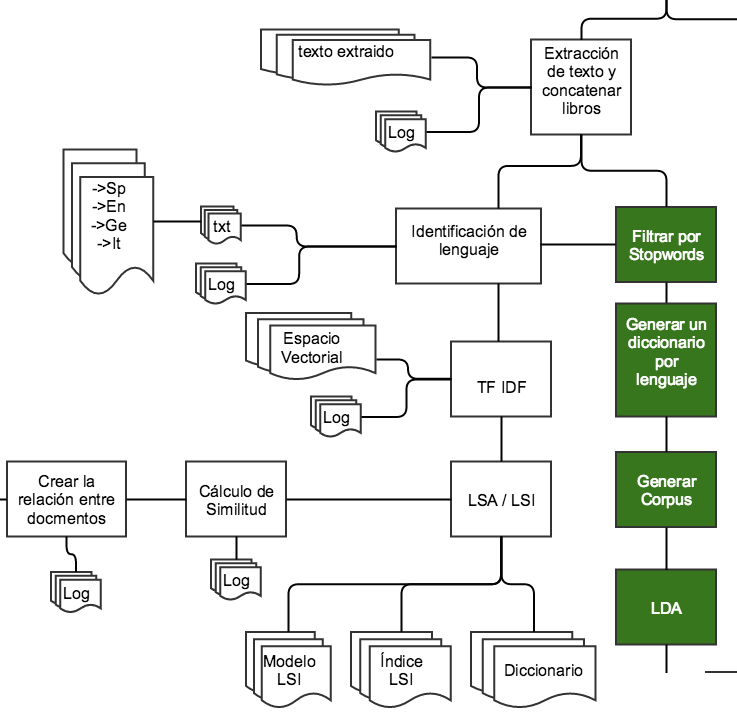
\includegraphics[width=0.6\textwidth]{Figures/pipeline_text.png}
\caption{Pipeline procesamiento de texto}
\end{figure}

La idea es que el usuario pueda explorar la colección de una manera más amigable que un simple listado de  libros. Los resultados del LDA permiten explorar grupos de libros similares a través  términos comunes entre ellos, mientras que el análisis de similitudes (TF-IDF) permite encontrar rápidamente los libros de la colección que sean parecidos al elegido inicialmente.

En principio, estos procesos serán completamente automáticos (salvo la elección de algunos parámetros descritos posteriormente) y le ahorrarán mucho tiempo a los expertos. En las siguientes secciones de este capítulo se describen a más detalle todos los componentes.\\

\textbf{Nota:} Tanto el equipo de la UNAM/ GIL como el equipo del ITAM usaron TF-IFD, dado que el equipo de la UNAM son los expertos en Lenguaje Natural se decidió utilizar el suyo en el flujo del proyecto.

\section{Vectorización de textos}

Antes de hacer los modelos es necesario convertir los datos no estructurados (es decir, los textos crudos de los libros) en datos estructurados. La técnica más común en minería de textos consiste en realizar conteos de palabras por documento y acomodarlos en una matriz. Conceptualmente, se construye la \emph{matriz términos-documentos} (TDM) $T$ como una matriz de entradas enteras de dimensión \emph{número de términos o palabras ($M$)} $\times$ \emph{número de documentos ($N$)}, con entradas:

$$
T_{w,d} = \text{número de veces que aparece el término } w \text{ en el documento (libro) } d
$$

Con la creación de la TDM se pierde el orden de las palabras en los libros, pero se mantiene la información estadística de las apariciones de las mismas. En principio, el número de términos debe coincidir con el número de palabras observadas en la colección, pero esto hace ruidosa la búsqueda ya que contabiliza todos los tiempos de los verbos. Por ejemplo, en este caso no se toma en cuenta que las palabras ``comer'', ``comen'' y ``comemos'' en realidad significan lo mismo y deberían tomarse en cuenta como una aparición del verbo ``comer''. Para tratar con este problema se hizo lo siguiente:

\begin{enumerate}
    \item Se separó la colección en varias subcolecciones, una por cada idioma disponible. Esto tiene sentido porqué cualquier asociación encontrada entre libros en diferentes idiomas puede ser considerada ruido y además puede hacer más lento el análisis. Todos los procesos subsecuentes se hicieron por separado en cada idioma.
    \item Se aplicó la técnica \emph{stemming} para disminuir el ruido de los términos, esta técnica consiste en utilizar la raíz de la palabra en lugar de la palabra misma, en el ejemplo de ``comer'', ``comen'' y ``comemos'' las contabiliza como la misma palabra (raíz ``come''). Hay varios algoritmos que hacen esto, pero dado el tamaño de la colección y por sugerencia del equipo de la UNAM, se hizo un \emph{stemming} simple truncando las palabras a una longitud máxima de 6 caracteres.
\end{enumerate}

De este modo, la TDM $T^{idioma_i}$ en realidad tiene un renglón por cada término de a lo más 6 letras encontrado en la colección en el $idioma_i$. 

\textbf{Nota:}En lo sucesivo se omitirá el idioma para facilitar la exposición, pero debe sobre entenderse que los análisis se hicieron por separado.

\section{Term Frequency – Inverse Document Frequency (TF-IDF) }

Para obtener una medida de similitud entre los documentos se aplicaron varias técnicas. En esta sección se explica la primera, que consiste en una transformación de la matriz $T$ para obtener similitudes. Para simplificar la notación, denotaremos por $T_d$ al vector de todas las frecuencias de los términos conocidos del documento $d$ y por $T_{w,d}$ las entradas de $T$ como están definidas en la sección anterior.

Supongamos que queremos comparar los documentos $q$ y $d$. Un primer enfoque que podríamos utilizar sería usar la similitud coseno, que toma en cuenta únicamente la frecuencia relativa de las palabras dentro de los documentos:

$$
sim(q,d) = \frac{T_q \cdot T_d}{\|T_q\| \|T_d\|}
$$

El problema con lo anterior es que las palabras comunes podrían tomar un papel fundamental y en nuestro caso compartir, por ejemplo, artículos o preposiciones no es muy interesante. Para mitigar esto se utilizó la frecuencia inversa en documentos $idf_w$, definida para una palabra $w$ como sigue: si $N$ es el número total de documentos en la colección y $df_w$ es el número de documentos de la colección que contienen a $w$, entonces definimos la frecuencia inversa de documentos como sigue:

$$
idf_w = log(\frac{N}{df_w}) 
$$

Entonces, en lugar de describir a $d$ por medio de $T_d$, lo describimos por medio de $c_d$, donde

$$
c_{d,w} = idf_w \times T_{d,w}
$$

Y así, calculamos la similitud entre dos documentos como el coseno entre sus vectores característicos:

\begin{align} \label{f:simcos}
sim(q,d) = \frac{c_q \cdot c_d}{\|c_q\| \|c_d\|}
\end{align}

La $idf_w$ es el logaritmo del inverso de la probabilidad de que el término $w$ aparezca en un documento elegido al azar. 
Las consecuencias de esto es que las palabras comunes casi no tendrán ningún efecto en la distancia, puesto que su probabilidad es cercana a 1 y por lo tanto su $idf$ es cercana a cero. 

Por el contrario, las palabras raras tendrán una probabilidad cercana a 0, por lo que su $idf$ será grande y contribuirán mucho. 
La idea detrás de este proceso es que se quiere que se utilice las palabras especiales o específicas a un contexto para discriminar, no las genéricas.
El esquema expuesto está escrito con mayor detalle en el libro \href{http://www.mmds.org}{Mining of Massive Datasets} ver \citep{leskovec2014mining},
con la pequeña diferencia de que nosotros no normalizamos $T_w$ por la máxima frecuencia obtenida por el término en la colección de documentos.


%%%% cambiar redacción 
Si bien se obtiene mucho mejores resultados utilizando la matriz $C = [c_1, \dots, c_N]$ es mucho más eficaz que si se utiliza la matriz $T$, aún hay ciertos elementos ruidosos que se puede mitigar. Para ello presentaremos la siguiente técnica.

\section{Latent Semantic Indexing (LSI)}

El Análisis de Semántica Latente (o LSI por sus siglas en inglés) es una técnica que se puede utilizar para refinar  más la similitud entre documentos calculada con TF-IDF.
Principalmente lo que hace es quitar el ruido de las palabras con muchos significados y de los términos con el mismo significado.
Para ello, encuentra los términos latentes u ocultos que conceptualmente tienen la mayor cantidad de información 
posible y los utiliza en lugar de las palabras normales.

Esta técnica fue propuesta por la UNAM y está explicada con mayor detalle en su documentación hermana, 
la idea general consiste en obtener la Descomposición en Valores Singulares (SVD) 
de la matriz TF-IDF y truncar los valores singulares pequeños,
dejando únicamente un número pequeño en comparación con el rango de la matriz (digamos, algún número entre 100 y 300).
Expresado matematicamente si la SVD de $C$ es 
$C = U \Sigma V^T$ \\

y $\Sigma_k = \Sigma$\\

una vez que se truncaron a cero todos sus valores singulares, a excepción de los $k$ más grandes, 
entonces se puede aproximar $C$ con $C_k = U \Sigma_k V^T$, donde
$C_k$ tiene rango $k \leq rango(C)$ y, por lo tanto, menos
efectos ruidosos que $C$. El LSI consiste en calcular las
similitudes como en la ecuación (\ref{f:simcos}), pero 
utilizando la matriz $C_k$ en lugar de $C$. En \citep{rosario2000} viene el proceso con más detalle.

Un factor importante para que funcione el LSI es el número de dimensiones latentes $k$ a utilizar. 
De preferencia debe ser elegido mediante validación por un
experto, que pueda evaluar los resultados obtenidos con diversos
valores de $k$ y elegir el que dé similitudes más coherentes. 
En la sección de resultados está explicado qué hace el programa para ayudar al experto a elegir $k$ de manera apropiada.


\section{Latent Dirichlet Allocation (LDA)}

A través de modelación de tópicos es posible analizar grandes cantidades
de datos sin categorizar cada uno por separado. Uno de los métodos más populares modelar tópicos es
LDA (Latent Dirichlet Allocation)  por sus cifras en inglés.
Es importante mencionar la propiedad de conjugación dadas las siguientes
distribuciones: Si tenemos:

\[ \phi \sim Dir(\alpha) \] \[ W \sim Mult(\phi) \] y
\[ n_k = |\{w_i:w_i = k \}| \] entonces
\[ P(\phi|\alpha, W) \propto P(W|\phi)P(\phi|\alpha) \]
\[ \propto \prod_k \phi^{n_k} \prod_k \phi^{\alpha_k-1} \]
\[ \propto \prod_k \phi^{\alpha_k+n_k-1} \]

Es decir son conjugadas, por lo que la distribución posterior tiene la
misma forma que la distribución a priori y en nuestro caso sólo estamos
agregando las observaciones. Ahora es más sencillo comprender la función
de LDA, el cual es un modelo generativo que asume:

\begin{enumerate}
  \item Cada tópico $k \epsilon \{1,...,K\}$ es una mezcla de palabras que tiene una distribución multinomial $\beta_k$ la cual proviene de una distribución de Dirichlet con parámetro $\lambda$. 
    \item Cada documento $d \epsilon \{1,...,M\} $ es una mezcla de tópicos con distribución multinomial $\sigma_d$ la cual proviene de una distribución de Dirichlet con parámetro $\alpha$.
    \item Para cada palabra $n \epsilon \{1,...,N\}$, se selecciona un tópico escondido (variable latente) $Z_n$, los cuales provienen de una distribución multinomial parametrizada por $\theta$.
\end{enumerate}

El modelo está representado por la figura \ref{lda}:

\begin{figure}[H]
\centering
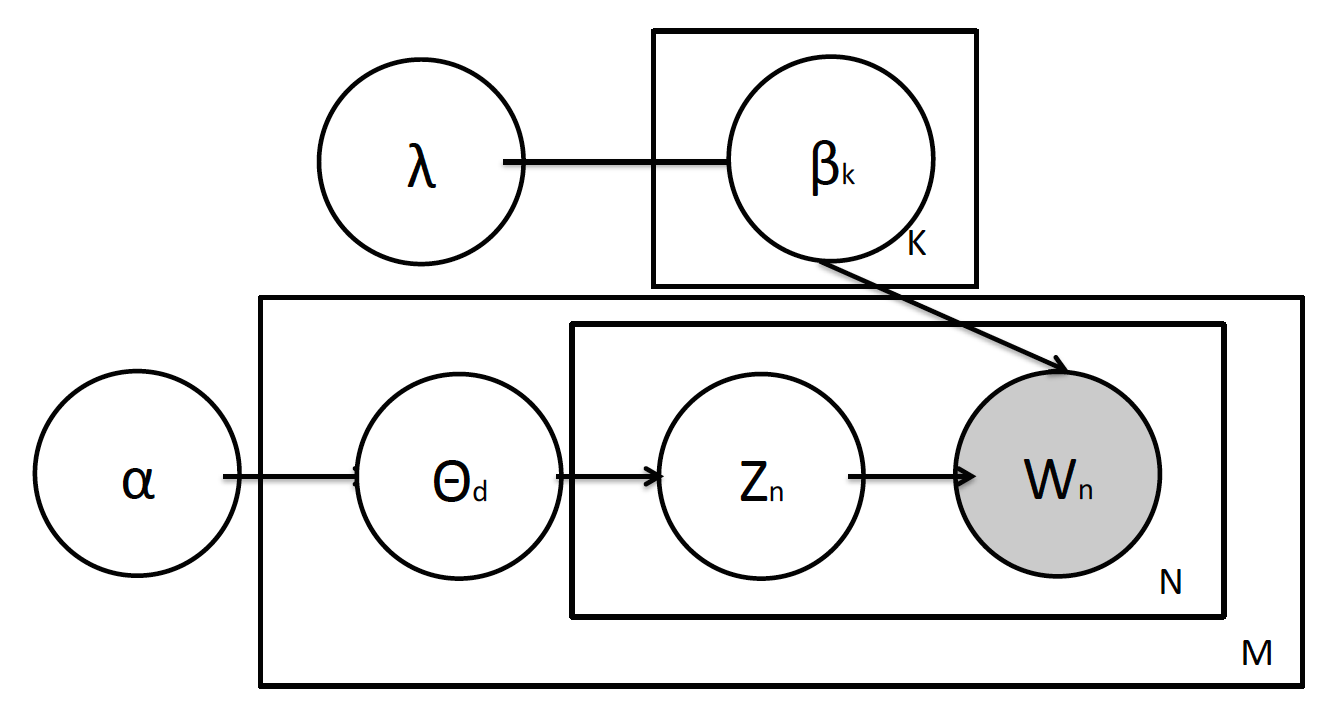
\includegraphics[width=.6\textwidth]{Figures/lda.png}
\caption{LDA}
\label{lda}
\end{figure}

Cada palabra observada está asociada con uno y sólo un tópico. Con base en esta idea y diagrama, es posible generar la palabra observada, es decir el tópico que le corresponde al documento.  A través de inferencia estadística descubriremos las variables latentes más probables, en nuestro diagrama las $Z_n$, las cuales explican de mejor manera nuestro conjunto de datos que nos va a decir cuáles son las $\beta_k$ y las $\theta_d$.
\vspace{0.5cm}

\noindent Para poder determinar los tópicos adecuados vamos a utilizar el muestreo de Gibbs (Gibbs sampling). Esto se logra a través de el cambio en la asignación de tópicos a cada una de las palabras $Z_{d,n}$ ya que comenzamos con asignaciones de tópicos de forma aleatoria y queremos ir mejorando estos tópicos de forma gradual hasta que tengan sentido. Es decir, dado un estado $\{Z_1, ..., Z_N\}$, tenemos que $Z_n \sim p(n_n|Z_1,...Z_{n-1}, Z_{n+1},..., Z_N, X,\Theta)$, y esto lo hacemos con repetición para todas las palabras en nuestros documentos.
\vspace{0.5cm}



\noindent Se inicia asignando tópicos a todas las palabras de todos los documentos y de forma sistemática se reasignan los tópicos a las palabras,  esto se hace de manera iterativa y cada vez se muestrea  la asignación de tópicos de una de las palabras basado en la asignación de las demás para todas las palabras, véase figura \ref{fig:Gibbs_sample}. Integrando al modelo las demás variables correspondientes a los parámetros $\alpha$ y $\lambda$ a través de Rao-Blackwellized \citep{Canini} ya que nos interesa:

\[ p(Z_{d,n}=k | Z_{-d,n}, w, \alpha, \lambda)= \frac{p(Z_{d,n}=k, Z_{-d,n}| w, \alpha, \lambda)}{p(Z_{d,n}| w, \alpha, \lambda)} \]


\vspace{0.5cm}

haciendo los  cálculos se tiene,

\[ p(Z_{d,n}=k | Z_{-d,n}, w, \alpha, \lambda)= \frac{n_{d,k}+\alpha_k}{\sum_{n=i}^{K}n_{d,i}+\alpha_i} \frac{v_{k,w_{d,n}}+\lambda_{w_{d,n}}}{\sum_i v_{k,i}+\lambda_i}\].



En dónde $n_{d,i}$ es el número de palabras que tienen el tópico $i$ en el documento $d$ y $v_{k,w}$ es el número de veces que la palabra $w$ se usa en el tópico $k$. Por lo que el proceso de remuestreo se puede dividir en dos partes y contar en dos partes:


\begin{figure}[h]\centering
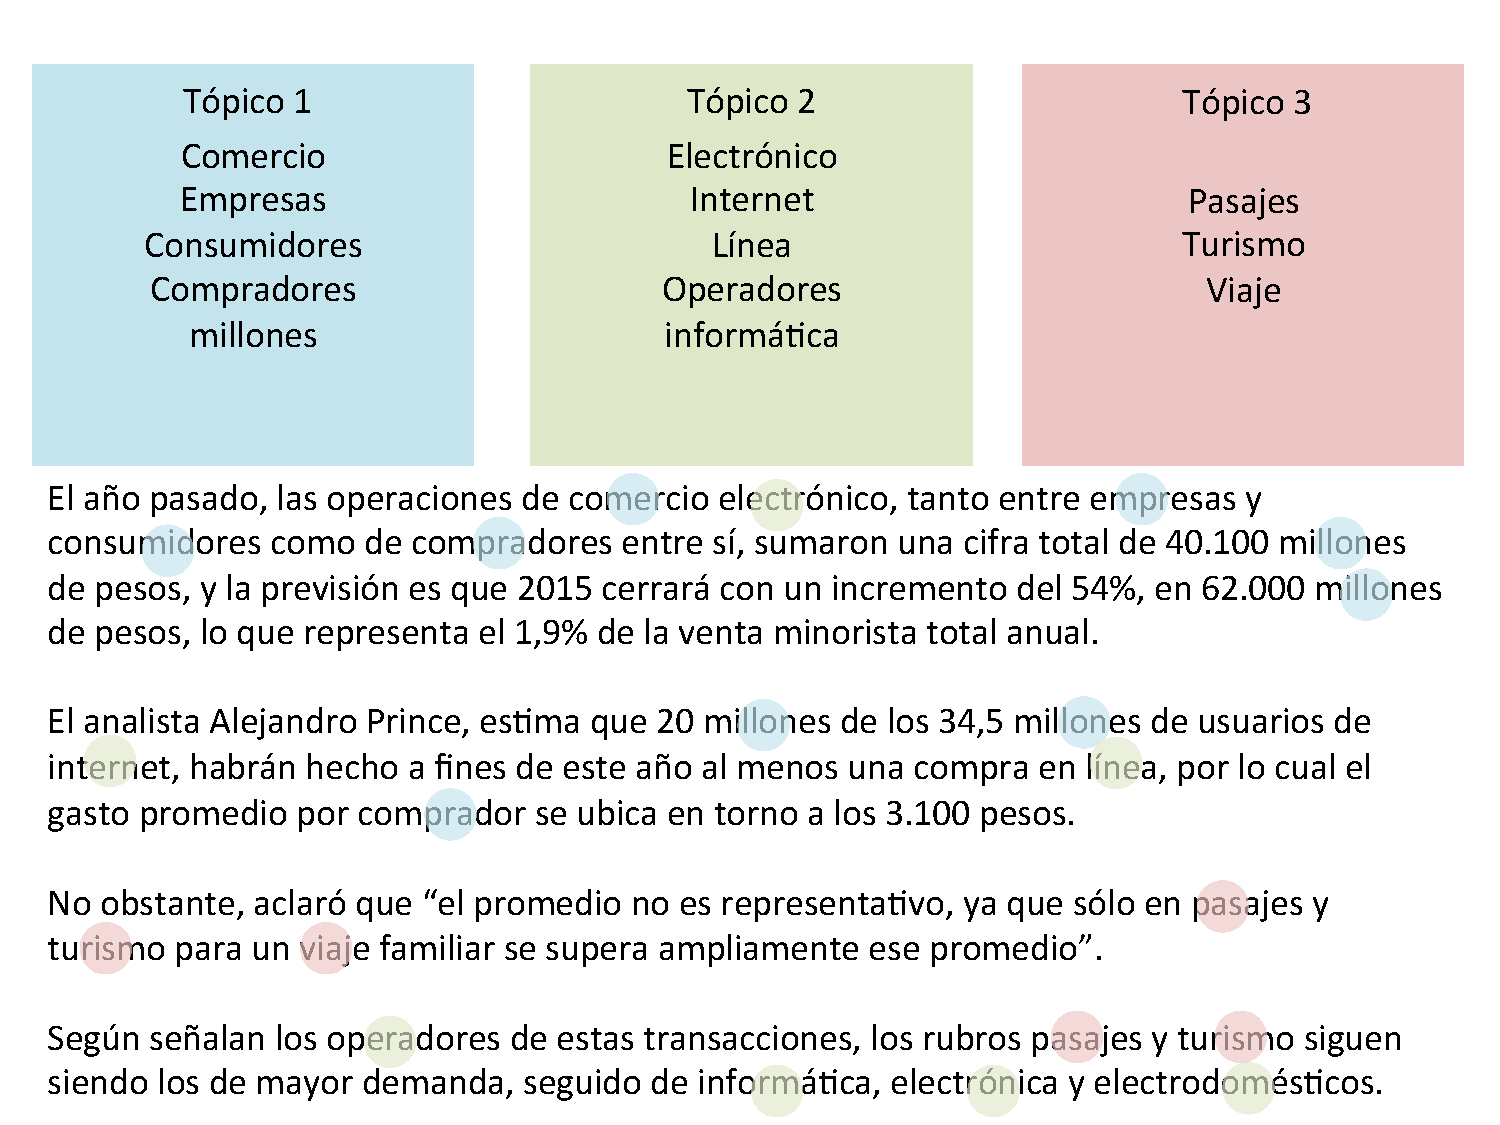
\includegraphics[width=12cm]{gibbs_sampling.pdf}
\caption{Muestreo de Gibbs}
\label{fig:Gibbs_sample}
\end{figure}

\newpage

\begin{enumerate}
  \item ¿Qué tantas veces aparece cada tópico en casa documento?
  \item ¿Qué tanto aparece cada palabra en cada tópico?
\end{enumerate}

Por lo que al multiplicar los valores obtenidos para cada una de las partes tenemos el valor proporcional de la probabilidad de asignación de los tópicos para la palabra que escogemos, y de esta manera vamos armando la mezcla de tópicos para cada documento, ver Figura \ref{fig:mezcla_topicos}


\begin{figure}[h]\centering
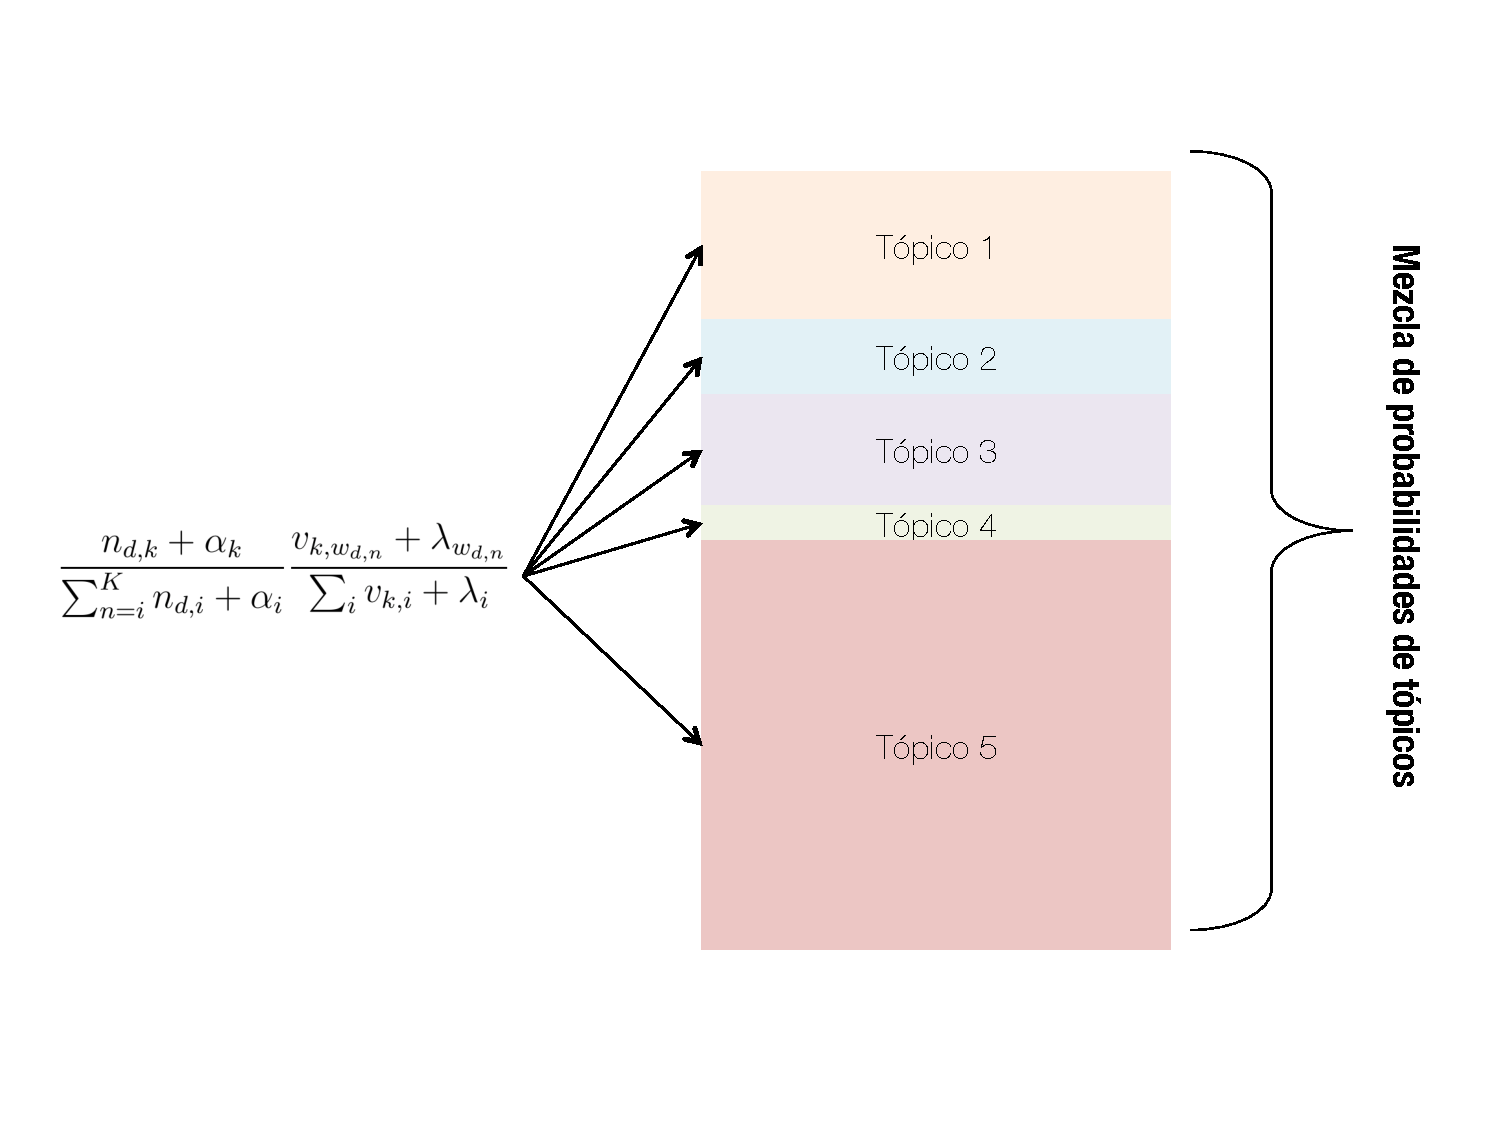
\includegraphics[width=12cm]{mezcla_topicos.pdf}
\caption{Mezcla de tópicos}
\label{fig:mezcla_topicos}
\end{figure}



\noindent El objetivo de encontrar los tópicos en la colección de texto es hacer una partición la cual nos permite identificar grandes bloques de temas. Esto se hace con el objetivo de poder buscar una colección o tema en particular dentro del catálogo. 



\section{Elección de parámetros} %No sabemos si es sección

En esta sección se explica el criterio para elegir los parámetros que permiten la implementación de distintos algoritmos los cuales son parte del pipeline. Existen parámetros que se deben elegir manualmente y se heredan a todos los procesos. 

\begin{itemize}
	\item Idiomas. 
	\item Nivel de limpieza.
\end{itemize} 

Es importante mencionar que se realiza la extracción y limpieza de todos los libros, y posteriormente sólo se realizan los modelos de los idiomas que se escogen.
\vspace{0.2cm}

\noindent Los parámetros a escoger que corresponden a LDA (modelación de tópicos automática) son:

\begin{itemize}
	\item Número de tópicos: Este parámetro corresponde a la cantidad de \textit{clusters} o nivel de partición del conjunto de libros. A mayor número de tópicos, mayor especificidad en  la asignación.
	\item El número de pasadas al texto: Este parámetro está implementado en el código, 
	sin embrago este es fijo a 10 ya que valores más altos implican un costo computacional más alto.
	Este parámetro puede ser explorado en un futuro para medir la ganancia en la especificidad de los tópicos.
\end{itemize}


Como se mencionó anteriormente un experto debe elegir los valores a utilizar. Para ayudarle a tomar la decisión, se generó un archivo en HTML que presenta los resultados como se muestra en la siguiente figura \ref{fig:outputLDA} :
\vspace{0.2cm}


\begin{figure}[h]\centering
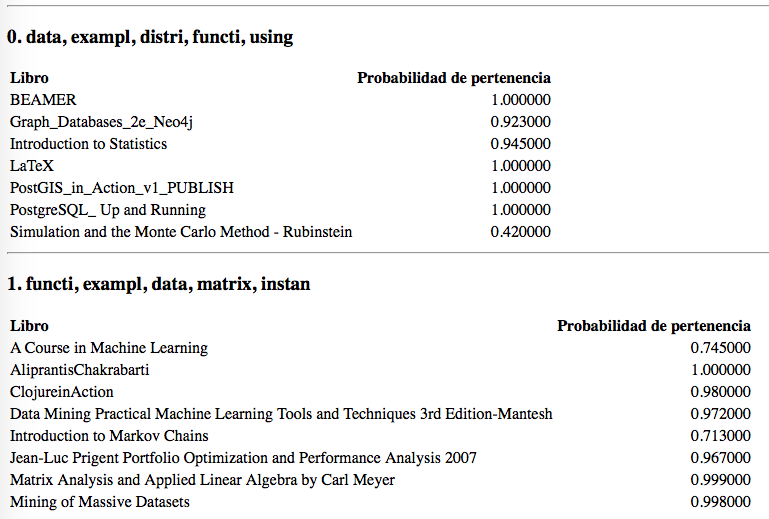
\includegraphics[width=5cm]{htmlLDA.png}
\caption{Salida en HTML de LDA}
\label{fig:outputLDA}
\end{figure}


\vspace{0.2cm}
El parámetro a escoger que corresponde a LSI (similitud entre libros) es:

\begin{itemize}
	\item Número de dimensiones latentes: Mientras más grande es este parámetro el criterio es más preciso, pero más ruidoso. Hay que probar varios valores para encontrar el nivel de especificidad óptimo. 
\end{itemize}


De manera similar presentamos los resultados en un archivo HTML el cual facilita la toma de decisión respecto al valor del parámetro mencionado anteriormente como se muestra en la siguiente figura \ref{fig:outputLSI}
\vspace{0.2cm}

\begin{figure}[h]\centering
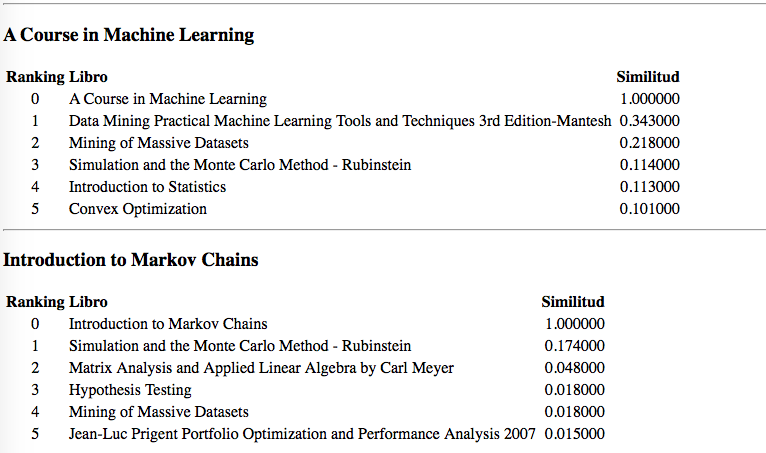
\includegraphics[width=5cm]{htmlLSI.png}
\caption{Salida en HTML de LSI}
\label{fig:outputLSI}
\end{figure}




\section{Conclusión}
El procesamiento de texto es sin duda, un análisis fundamental para encontrar patrones de asociación dentro de la colección de textos disponible y textos por agregar. Como se mencionó anteriormente, este proceso permitirá que el usuario pueda realizar búsquedas bajo distintos criterios ya sea por similitud en cuanto al texto, como lo permite la búsqueda por LSI, o en cuanto a temas en particular como lo permite la búsqueda por LDA.

El desarrollo del procesamiento de texto mediante una gestión de pipelines a través de \texttt{luigi} impulsa un ecosistema de producción sano, ya que existen procesos que por naturaleza son computacionalmente costosos y por lo tanto tardados los cuales pueden ser paralelizados y gestionados si es que existen errores. 
En particular dentro del pipeline de procesamiento de texto,  la limpieza es un proceso tardado, 
sin embargo con \texttt{luigi} es posible realizar esta tarea en paralelo y si existe un error en algún momento, no es necesario volver a generar toda la información desde cero, s
i no que retomamos el proceso a partir de dónde se generó el error. Por otra parte se genera la información necesaria una sola vez, la cual sirve para generar los modelos de LSI y LDA.

\section{Problemas}

Algunos de los mayores problemas encontrados a lo largo del desarrollo consistieron en el manejo de los hiper-parámetros del modelo, uno de estos consiste en el número de pasadas al texto el cual en cierto rango mejora el modelo. Este hiper-parámetro influye directamente con el tiempo de procesamiento de los datos. También se deja al criterio del usuario la selección del número de tópicos ya que esto depende del nivel de partición de la colección que se desee. Entre más tópicos, más específico es el subconjunto de selección, por esto es importante que el experto especifique el nivel de partición. Los tópicos están determinados por una combinación lineal en la que los escalares son la probabilidad de pertenencia de cada tema ($0.83 México + 0.65 dibujo + 0.55 paisaje + 0.5 Velasco$) . Es por esto que es importante que el experto determine un único tópico para esta combinación.

En general, el reto consistió en la construcción de un pipeline óptimo para el procesamiento de texto. Dado que existen procesos que tienen dependencias compartidas, fue fundamental la implementación a través de un esquema de pipelines como lo permite  \texttt{luigi} ya que se paralelizó el trabajo en ciertos procesos como lo fue la limpieza de datos y por otra parte se generó la información una única vez como lo es para el corpus y el diccionario, ya que estos fueron utilizados tanto para el desarrollo y generación de similitudes a través de LSI y el modelado de tópicos a través de LDA.

La presentación de resultados para la toma de decisión de los parámetros fue analizada y evaluada para ser presentada de forma sencilla ya que para el procesamiento interno solamente era necesario guardar los datos en una etapa del proceso en un formato de Python llamado \textit{pickle} el cual nos permite guardar los datos en forma binaria. Sin embargo, para conseguir un producto final en el que un experto determine los metaparámetros de los algoritmos, fue necesario determinar el formato más amigable para presentar los resultados obtenidos. En la sección \textit{Elección de parámetros} se menciona de forma detallada su interpretación. 

\section{Trabajo futuro}

Una manera de ampliar los resultados anteriormente expuestos, consiste en los siguiente:

\begin{enumerate}

	\item Reentrenamiento con datos nuevos: Por el momento es posible asignar una mezcla de tópicos a los documentos nuevos basado en el modelo LDA base. Sin embargo dado que la colección de textos incrementará con el tiempo, es altamente recomendado reentrenar el modelo de LDA ya que este contará con más información y probablemente con más tópicos. 
	\item Procesamiento en paralelo: A medida de que la colección crezca, es posible generar un modelo de LDA a través del procesamiento paralelo, esto con la finalidad de disminuir el tiempo de entrenamiento del modelo.
	\item Nuevas características y algoritmos: Dentro del procesamiento de texto es posible encontrar entidades véase \footcite{https://en.wikipedia.org/wiki/Named-entity_recognition}, por lo que se contempla en un futuro poder emplear este tipo de técnicas para encontrar relaciones entre entidades. 
	
\end{enumerate}



	\chapter{Procesamiento de Imagen}
\label{cap_im}
\section{Introducción}

Este proceso busca analizar las páginas de libros escaneados por parte de OCRMX  a través de un análisis de los colores que componen las imágenes. Dado que la colección es de arte y principalmente se compone de  libros de pintura y escultura, entre otros,  creemos que es relevante que el usuario  pueda buscar por similitud en texto y en imágenes. 


Para ello, el proceso se descompone en tres partes:  la primera es identificar aquellas páginas que tienen una pintura dentro de la página; la segunda, analizar los colores   que  componen las pinturas  y tercera, identificar aquellas páginas con pinturas similares por la composición de sus colores.

El resultado final es un listado de todas las imágenes que tienen otra imagen similar, de acuerdo a su composición cromática, en formato XML, que permite hacer recomendaciones a aquellos que consultan el catálogo sobre otros libros que tienen imágenes similares.

Se probaron diferentes técnicas y métodos para poder conseguir cada uno de los subprocesos necesarios para alcanzar el objetivo. En las siguientes secciones se describe con mayor detalle los métodos para cada uno de los procesos para encontrar  imágenes similares.  En general se puede resumir en lo siguiente:

\begin{enumerate}
\item Definir una colección fija y reducida de colores y transformar los píxeles de cada imagen al color más cercano a esta colección.
\item Analizar cada página e identificar si la página tiene una imagen e identificar la composición cromática de la imagen.
\item Una reducción de las imágenes identificadas en el proceso anterior a una dimensión de 200 x 300, dado que la alta calidad de las originales hace muy complicado analizarlas en su forma inicial.
\item Construir de una matriz en donde las columnas representan cada uno de los colores definidos en el paso 1, cada renglón representa una imagen y cada cuadro de dicho renglón representa el conteo de píxeles en la imagen que pertenecen al color definido por la columna.
\item Encontrar imágenes similares a través del algoritmo de Local Sensitive Hashing(LSH) que permite de manera eficiente y rápida encontrar aquellas imágenes parecidas, tomando como medida de similitud la distancia coseno entre los vectores del conteo de colores.
\end{enumerate}

El diagrama de flujo de esta sección es el siguiente : 

\begin{figure}[H]
\centering
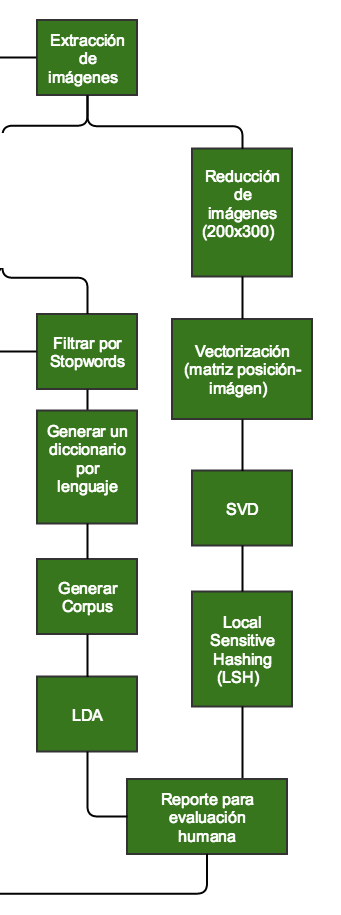
\includegraphics[width=0.3\textwidth]{Figures/pipeline_itam.png}
\caption{Pipeline procesamiento de imágenes}
\end{figure}


\section{Definir una colección fija y reducida de colores}

Para entender éste proceso y los subsecuentes se debe entender la forma por la cual las computadoras leen una imagen. Para esta acción existe un paradigma conocido como RGB, el cual descompone un color en tres capas: rojo, verde y azul, RGB por sus siglas en inglés. En cada una de estas capas existe un valor numérico que representa la intensidad de dicha capa, es decir la intensidad de azul, verde y rojo.  Cualquier color puede ser recreado como una combinación de estas (ver \cite{susstrunk1999standard}).


\begin{figure}[H]
\centering
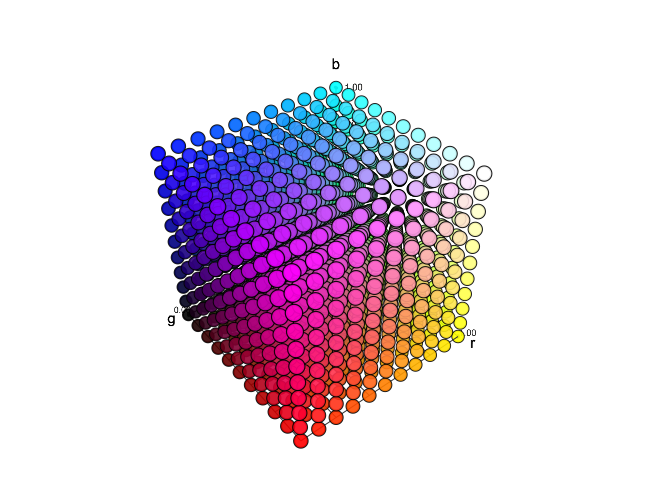
\includegraphics[width=1\textwidth]{Figures/cubo.png}
\caption{Espacio RGB}
\label{fig:cubo-rgb}
\end{figure}

Éste paradigma se ve reflejado en la figura \ref{fig:cubo-rgb}, en la cual se puede ver un cubo formado por distintos valores de rojo, verde y azul. Para este ejemplo, estos valores pueden ir del 0 al 1, representando este número la intensidad de cada capa, sin embargo, existen otras representaciones del paradigma en donde el valor puede ir de 0 a 256.

Respecto a las imágenes, estas se componen de píxeles, estos son pequeños puntos de colores que al aglomerarse forman la imagen. Toda imagen es entendida por la computadora como una composición de 3 matrices, una matriz con las intensidades de rojos, una de verdes y otra de azules, cada casilla de la matriz representa un píxel de la imagen cuyo color, como se vio en el párrafo anterior, se forma de la combinación de las tres capas.

Ahora, como se explicó antes, cada color se forma por la combinación de tres valores, en algunas ocasiones estos valores van del 0 al 1 y en otras del 0 al 256. Para nuestro caso, solo van del 0 al 1. Esto significa que el color que se forma de la combinación 0.935 en rojo, 0.267 en verde y 0.478 en azul es diferente del formado por 0.936, 0.268 y 0.479, respectivamente. Aunque visualmente una persona no pueda distinguir ambos colores,  la computadora los entiende como diferentes. Esto es relevante porque si uno de los objetivos es identificar los colores que se encuentran en la imagen, pequeñas variaciones en los dígitos harán que la computadora identifique millones de colores dentro de una imagen,  complicado cualquier tipo de análisis posterior. 

Para solucionar esta dificultad, se decidió limitar el número de colores que puede tomar un píxel, y convertir cada color de cada píxel a uno de los colores predefinidos. Esto reduce el número de posibles de colores que pueden existir en una imagen. Para realizar este proceso era importante desarrollar un método eficiente que permitiera de manera rápida hacer la transformación de cada píxel de las página. Si tomamos en cuenta que una página digitalizada tiene alrededor de 6,000,000 píxeles, que hay en promedio 200 páginas por libro y son más de 3,500 libros digitalizados, es fácil darse cuenta de lo tardado que podría ser el proceso en caso de no reducir el universo de colores.
 %%%%%%%%%%%%% Esto salió de mí %%%%%%%%%%%%%%%%%%%%%%%%%%%%%%%%%%%%%%%%%%%%%%%%%%%%%%%%%%%%%%%%%%%%%%%%%%%%%%%%

De esta forma se decidió, que la manera más rápida, sencilla y eficiente, era limitar el número de dígitos que podría tener los valores para la intensidad de las capas de rojo, verde y azul por medio de un redondeo a un dígito. Para clarificar, si volvemos al ejemplo donde un color se compone por 0.935, 0.267 y 0.478 de las capas respectivas, un redondeo a un dígito resultaría en 0.9, 0.3 y 0.5, u en otro caso más complicado, intensidades de 0.9836474, 0.6494334 y 0.3349854 se reduciría a 1, 0.6, 0.3. Con una sencilla función de redondear a un dígito, es posible redondear las tres matrices de la imagen de un solo golpe, lo que lo vuelve un método  rápido y efectivo.

Esto hace que exista una cantidad limitada de colores posibles en una imagen y existe una manera eficiente y rápida de transformar los colores a este universo. En concreto, los colores posibles que se pueden tener al hacer este redondeo son 1331, que son las combinaciones de 11 posibles dígitos (0, 0.1, 0.2, 0.3, 0.4, 0.5, 0.6, 0.7, 0.8, 0.9, 1) en tres capas, estos colores se pueden ver en la figura \ref{fig:colores-definidos}.  Y para una comparación de la alteración que sufrió  la imagen con esta transformación, véanse las figuras \ref{fig:paisaje-sin} y \ref{fig:paisaje-con}, antes y después de la transformación respectivamente. Se puede ver que la transformación no altera en gran medida la percepción visual de los colores y ayuda en gran medida a reducir la complejidad del problema.

\begin{figure}[H]
\centering
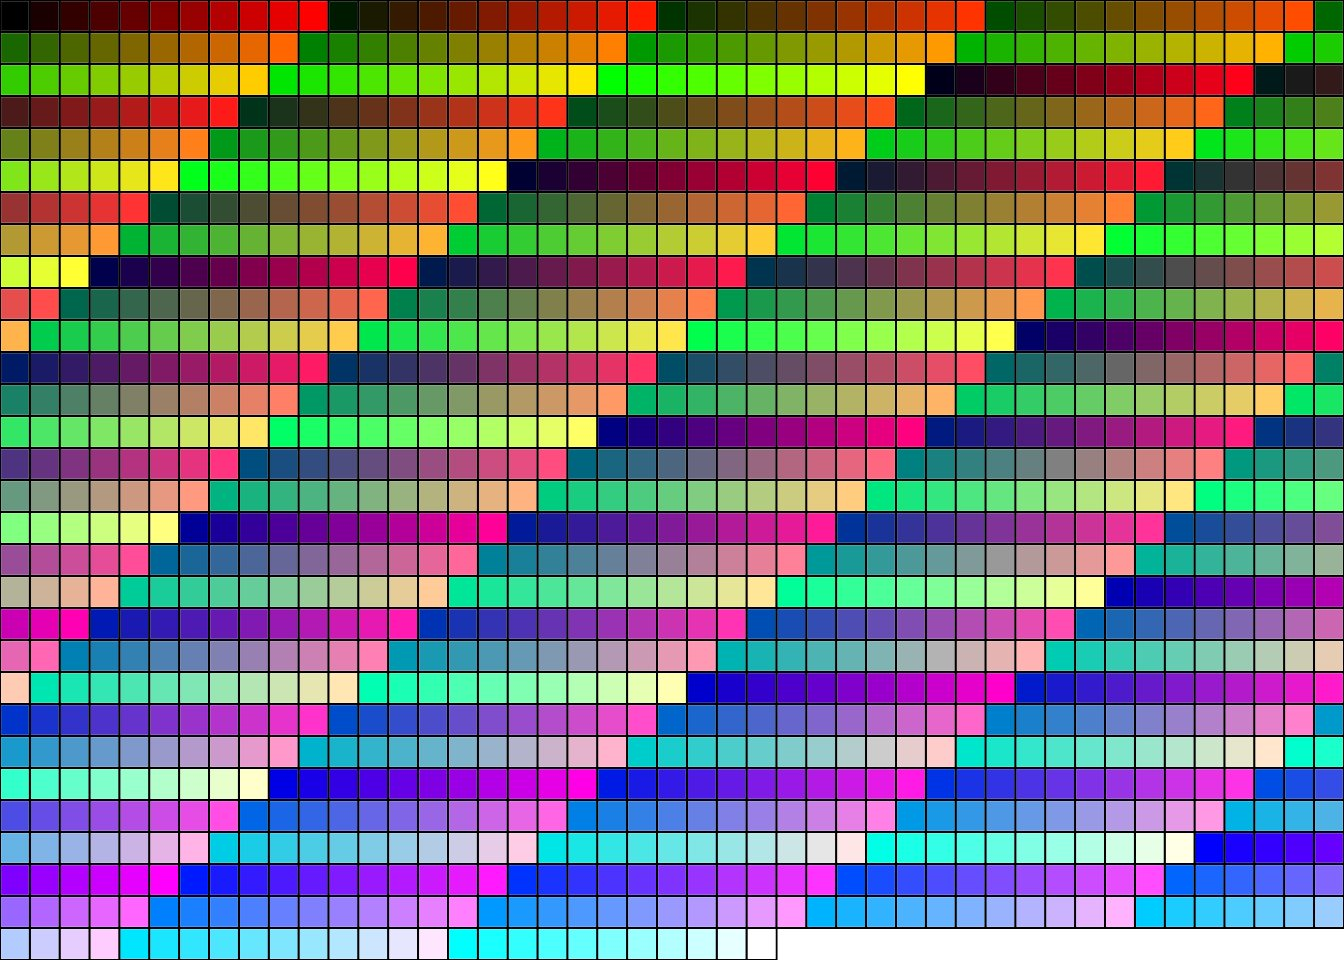
\includegraphics[width=0.8\textwidth]{Figures/colores_definidos.jpg}
\caption{Colores posibles en la imagen(1331).}
\label{fig:colores-definidos}
\end{figure}

\begin{figure}[H]
\centering
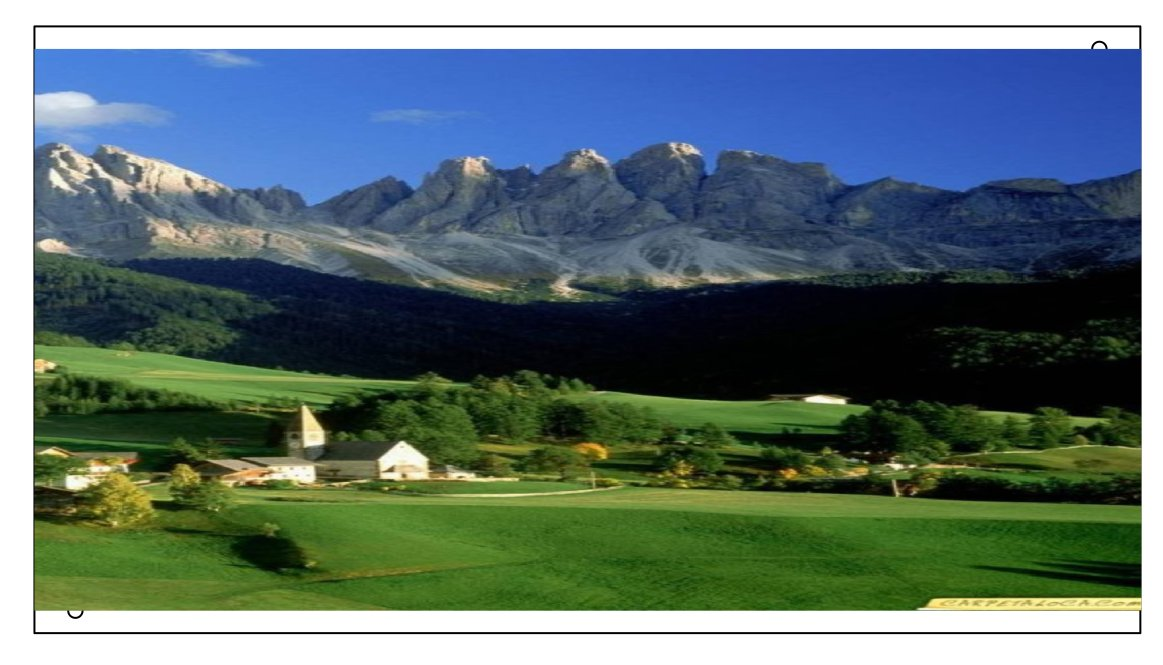
\includegraphics[width=0.8\textwidth]{Figures/paisaje_sin.jpg}
\caption{Paisaje sin alteración.}
\label{fig:paisaje-sin}
\end{figure}

\begin{figure}[H]
\centering
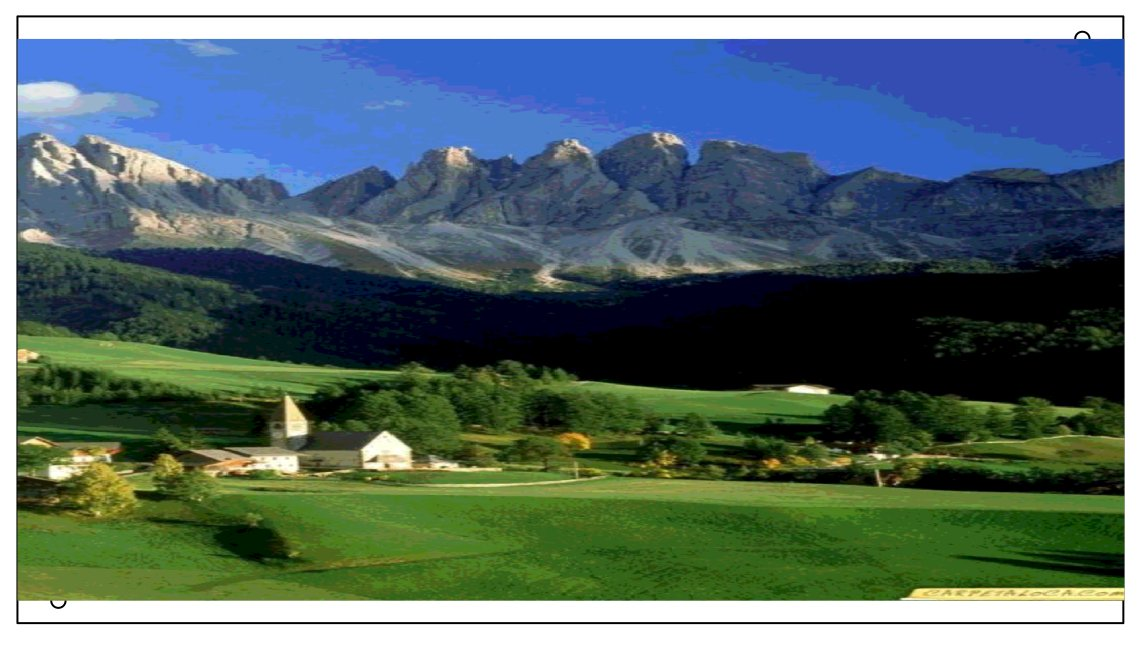
\includegraphics[width=0.8\textwidth]{Figures/paisaje_con.jpg}
\caption{Paisaje con reducción de colores.}
\label{fig:paisaje-con}
\end{figure}

\section{Identificar páginas con imágenes de colores}

El primer paso de éste proceso es  identificar  si una página contiene imágenes o no . Se realizaron pruebas para corroborar si la varianza de las matrices cromáticas de las imágenes eran de utilidad para dicho propósito. La colección de documentos contiene páginas en blanco, con texto monocromático, con texto multicromático y páginas con una o más imágenes, por lo que se espera que aquellas páginas que contienen imágenes tengan una mayor varianza que aquellas que solamente contienen texto. 


%%%%%%%%%%%%%%%%%%%%%%%%%%%%%%%%%%%%%%%%%%%%%%%%%%%%%%%%%%%%%%%%%%%%%%%%%%%%%%%%%%%%%%%%%%ME quedé revisando aquí 
 Para obtener la varianza de la imagen, no es necesario obtener esta con las tres matrices del RGB, es decir, la varianza de la página tendría que ser mayor incluso si la página estuviera en escala de grises. Es por ello que se decidió convertir las páginas a una escala de grises. Esto significa que ahora las imágenes no se componen de 3 capas de matrices, sino que ahora solo es una matriz, en la cual cada celda representa un píxel y el valor de dicha celda es la intensidad del negro, siendo 0 el blanco y el 1 el negro absoluto. Una vez transformadas las páginas en escalas de grises se saca su varianza, y si la varianza supera un número definido se considera que la página tiene una pintura dentro de la misma.

Para ilustrar mejor esta idea, véase la figura \ref{fig:varianza-sin} en donde estas páginas ya están en escala de grises y sus varianzas, de derecha a izquierda son 0.1074, 0.0515 y 0.0574. Se puede notar que existe una diferencia clara en las varianzas de la página de la izquierda respecto a la de la derecha, la cual solo contiene texto, sin embargo, la página de en medio tiene una varianza ligeramente menor que la de la derecha lo que indicaría que la varianza nos estaría ayudando para distinguir pinturas dentro de algunas páginas pero en otras fallaría.

\begin{figure}[H]
\centering
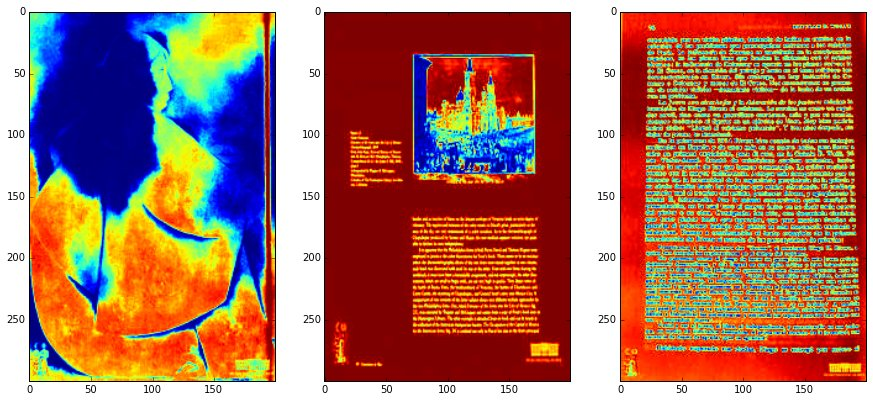
\includegraphics[width=1\textwidth]{Figures/prueba_varianza_1.jpg}
\caption{Identificación de imágenes sin filtro gaussiano}
\label{fig:varianza-sin}
\end{figure}

Para corregir este error, se usó un filtro gaussiano (ver \cite{burt1981fast}), que lo que hace es tomar un grupo de píxeles cercanos y promediarlos, esto hace que de alguna manera se difumina la imagen, como se puede ver en la figura \ref{fig:varianza-con}, pero al sacar la varianza ya con la transformación es mucho más útil para distinguir las páginas con contenido parecido a una pintura, ahora las varianzas son .0965, .0404 y .0146 respectivamente.

\begin{figure}[H]
\centering
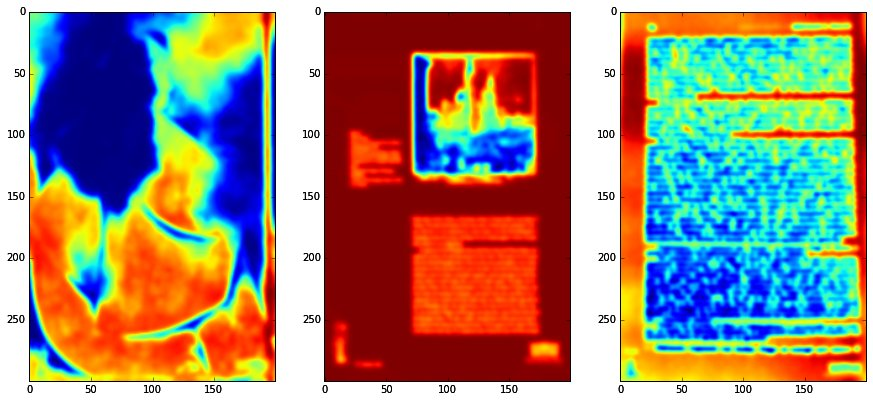
\includegraphics[width=1\textwidth]{Figures/prueba_varianza_2.jpg}
\caption{Identificación de imágenes con filtro gaussiano}
\label{fig:varianza-con}
\end{figure}

Avanzado el proyecto, con los resultados de las primeras pruebas, encontramos que existían muchísimos libros con imágenes en blanco y negro. En estos primeros resultados se encontraron muchas similitudes en imágenes en blanco y negro, aunque esto podría ser útil en alguna medida, el objetivo principal de este proyecto es sobre colores, por lo que decidimos enfocarnos en aquellas similitudes de imágenes a colores.

Para identificar las imágenes a colores se tuvo que idear un proceso por el cual al leer la página supiéramos si existen colores en esta o no, para después discriminar de nuestro análisis a las imágenes en blanco y negro. La manera más obvia para hacer esto es obteniendo la variedad de colores que existen en dicha imagen y si solo existen aquellos que van del blanco al negro, incluidos todas las escalas de grises, desecharlos y quedarnos con aquellas imágenes que tienen una mayor variedad de colores. Sin embargo, dado que son imágenes escaneadas, a pesar de que a simple vista las imágenes contenidas en las páginas fueran en blanco y negro, cuestiones de luz, basuritas microscópicas, entre otras cosas, hacían que incluso las páginas en blanco tuvieran una gran diversidad de colores.

Tal como usamos el filtro gaussiano para difuminar páginas previamente convertidas a escala de grises, se usó este filtro de nuevo para poder difuminar estas páginas pero ahora sin convertir a escala de grises, es decir se hizo el filtro sobre los tres canales del RGB.  Después de diversas pruebas para determinar cuál era la cantidad de colores diferentes necesarios para determinar si una imagen estuviera en color, se decidió el número de 100 colores diferentes como el límite. La figura \ref{fig:pruebas-colores} es parte de estas pruebas que se realizaron, estas ya tienen las 2 transformaciones mencionadas, una reducción de colores con el redondeo y el filtro gaussiano para los tres canales del RGB, en la parte superior de cada página se puede ver el número de colores diferentes que se encontraron en la página.

\begin{figure}[H]
\centering
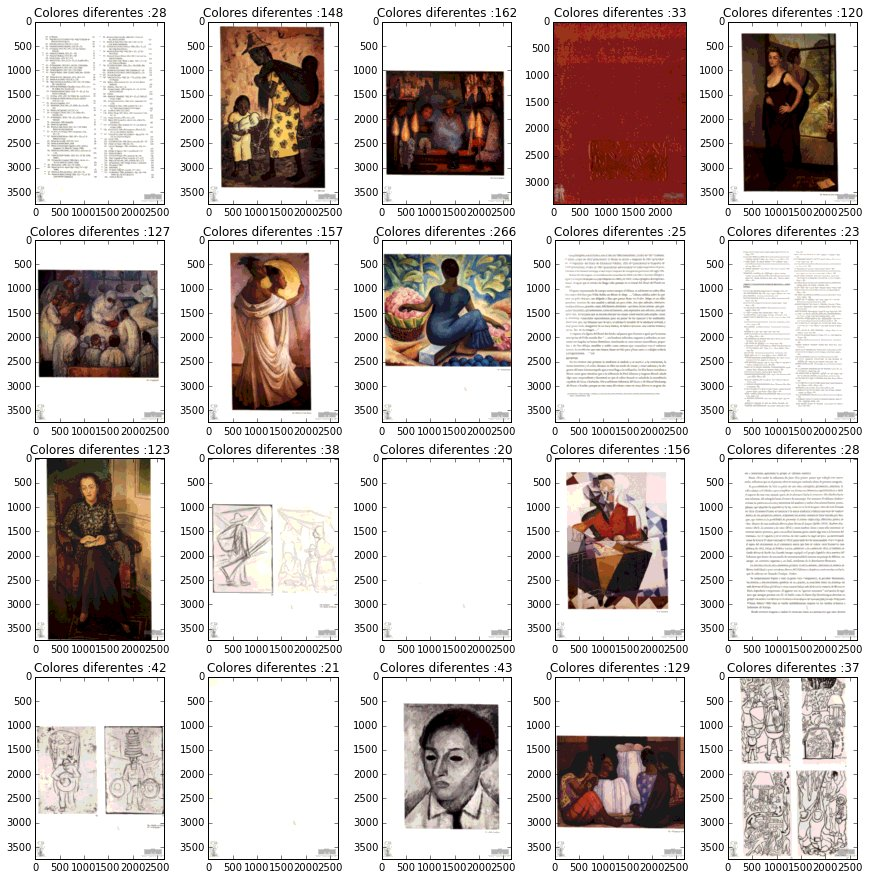
\includegraphics[width=1\textwidth]{Figures/identificar_colores.jpg}
\caption{Pruebas para determinar el número de colores mínimo}
\label{fig:pruebas-colores}
\end{figure}


Incluso, al realizar estas pruebas se percató que este procedimiento sirve para detectar qué páginas tienen imágenes dentro, por lo que el procedimiento de la varianza es reemplazado por este nuevo procedimiento de detección de color. Es decir, que el proceso de detección de colores  funciona a la vez para identificar imágenes porque entre más colores tenga la página mayor es la probabilidad de que sea por una imágen contenida en ella.

\section{Reducción de páginas a 200 x 300 píxeles}

La reducción de las imágenes obedece al hecho de que se tiene que realizar un conteo de los colores diferentes en cada página, este es diferente al que se realizó en el proceso pasado ya que en el anterior solo se buscaron los colores únicos, en este proceso se busca cuantos píxeles de cada uno de los 1331 colores definidos existen en la página. 

Las páginas escaneadas son de muy alta calidad, esta calidad es de alrededor de 2000 x 3000 píxeles, es decir que existen en la página cerca de 6 millones de píxeles, este número varía de pagina en pagina, pero en general no es muy distinto de este promedio. Dado lo anterior, hacer conteos sobre las páginas originales es muy tardado y ocupa mucha memoria RAM, por lo que para hacer el proceso más rápido y no desbordar la memoria se decidió hacer una reducción de aquellas páginas que se les detectó imágenes de colores. 

Este proceso se realiza con la librería de \texttt{Imagemagick} que corre sobre línea de comandos, particularmente se utilizó la función de  \texttt{mogrify} (ver \cite{still2005definitive}). Aunque la calidad de la imagen se pierde un poco, sigue siendo muy útil para realizar el análisis.

La figura \ref{fig:transformaciones} muestra el proceso por el cual se transformaron las imágenes, se debe mencionar que el filtro gaussiano no se incluye en esta transformación, ya que solo se utilizó para detectar imágenes pero la página no sufrió una modificación real. Cabe señalar que las originales se mantienen intactas, para aquellas que se realizan transformaciones permanentes se les hace una copia.

\begin{figure}[H]
\centering
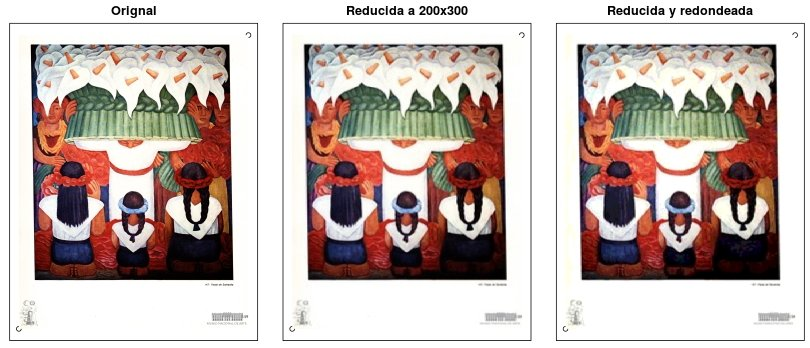
\includegraphics[width=1\textwidth]{Figures/transformaciones.jpg}
\caption{Proceso de modificación de imágenes, reducción y redondeo}
\label{fig:transformaciones}
\end{figure}

\section{Construcción de matriz de conteo de colores}

Como se mencionó en el apartado anterior, este proceso busca realizar un conteo de cada página de los colores que contiene, por lo que se abre cada página después de todos los procesos anteriores y se realiza un conteo de los colores, este conteo es transformado a un vector que es después consolidado a una matriz donde se están almacenando los conteos de todas las demás imágenes. Esta matriz tiene 1331 columnas que representan cada uno de los colores definidos, cada fila representa una imagen, y los datos en esta matriz son el número de píxeles que tiene cada imagen.

Se debe recordar que las imágenes que se analizan pertenecen a una página escaneada de un libro, por lo que es normal que la imagen no ocupe la página entera. 
Existe generalmente alrededor de la imagen un fondo blanco que puede hacer que el vector de colores esté muy cargado hacia este color, por otra parte, aunque se limitó el número de colores, todavía es suficientemente grande como para que existan diferentes tonalidades de un mismo color, es decir, que un color rosa de una flor,por ejemplo, va a tener diferentes tonalidades por los juegos de luces, lo que hace que se pulvericen los conteos de colores. Para tener más claro lo que se dijo veamos la figura \ref{fig:conteo-colores}, la cual es una página escaneada, si hacemos un conteo de sus colores y los representamos en una gráfica, se vería como la figura de en medio. 
El diámetro de las esferas representa la cantidad de píxeles que hay en dicho color, se puede notar que el color blanco es el preponderante, y que existe algunas esferas más chiquitas de colores diferentes, sin embargo se ven opacadas por el tamaño de los conteos de blanco. Si dejamos los vectores de conteo tal cual, va a ser afectado el algoritmo de similitud, ya que para determinar que tan parecidas son las imágenes toma en cuenta las proporciones de los colores, lo que resultaría en que todas las imágenes son parecidas ya que comparten en gran medida el blanco.

\begin{figure}[H]
\centering
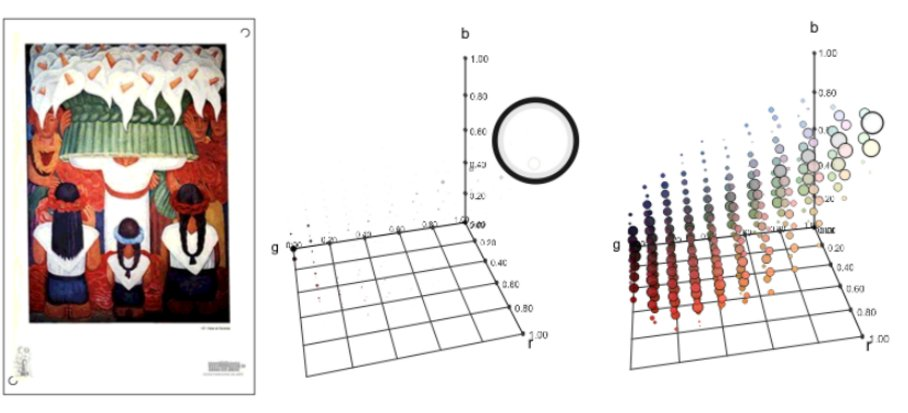
\includegraphics[width=1\textwidth]{Figures/conteo_colores.jpg}
\caption{Representación de conteo de colores}
\caption*{De lado izquierdo se encuentra la imagen escaneada después de reducción y redondeo de colores, en medio se encuentra la representación de conteo de colores en la dimensión RGB, de lado derecho está la representación del conteo pero después de sacar logaritmo natural.}
\label{fig:conteo-colores}
\end{figure}


Aunado a lo anterior, el fondo no debería contar dentro del conteo, ya que no es un color propio de la imagen, la solución ideal sería poder recortar el cuadro de la pintura para que el fondo no se incluyera dentro del conteo. Se realizaron pruebas con algoritmos de detección de esquinas para poder ver si era viable hacer este recorte de manera automática, este algoritmo no pudo identificar de manera clara las esquinas del cuadro ya que también detectaban esquinas dentro de la imagen, por lo que esta opción no se pudo seguir.

Para poder superar estas dificultades se utilizó en vez del conteo simple, el logaritmo del conteo, es decir, cada valor de la matriz se le aplicó el logaritmo natural para evitar que existieran valores tan disparatados, de esta forma el conteo de la imagen anterior ahora se vería como en la imagen de lado derecho de la figura \ref{fig:conteo-colores}. Se puede notar que el blanco deja de ocupar el lugar tan preponderante que tenía y que los colores tienen un mayor parecido con la imagen original.
 %%%%%%%%%%%%% Esto no lo tomé de nadie %%%%%%%%%%%%%%%%%%%%%%%%%%%%%%%%%%%%%%%%%%%%%%%%%%%%%%%%%%%%%%%%%%%%%%%%%%%%%%%%

\section{Encontrar imágenes similares}

Este es el proceso final, el que da como resultados las imágenes que se parecen. Una descripción más detallada del algoritmo de Local Sensitive Hashing lo podemos ver en un apartado más adelante, pero a grandes rasgos lo que busca es de manera rápida y eficiente determinar qué observaciones son parecidas de acuerdo a sus atributos. En el caso concreto de este proyecto una observación es una página de un libro con una imagen, los atributos de esta observación son el logaritmo del conteo de colores como se vio en el apartado anterior. La similitud la determinamos como la similitud coseno, que es una forma de calcular la similitud entre dos vectores (ver \cite{leskovec2014mining}).


Después de todos los procesos anteriores, se ejecutó el algoritmo de Local Sensitive Hashing y algunos de los resultados de este algoritmo de similitud son pares de imágenes que se encuentran en las figuras siguiente, las cuales tienen una similitud mayor al 90\% en sus colores. Es preciso mencionar que se debe juzgar su similitud no por el tema o las figuras de las pinturas, si no por la combinación de colores de las mismas.

\begin{figure}[H]
\centering
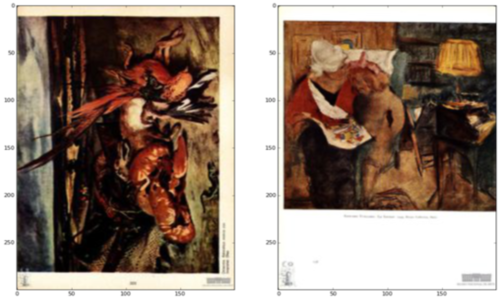
\includegraphics[width=0.8\textwidth]{Figures/similitud_1.png}
\caption{Par de imágenes similares 1}
\end{figure}

\begin{figure}[H]
\centering
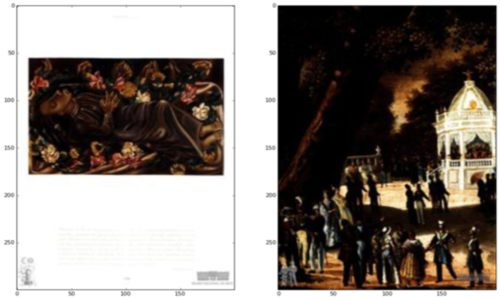
\includegraphics[width=0.8\textwidth]{Figures/similitud_2.png}
\caption{Par de imágenes similares 2}
\end{figure}

\begin{figure}[H]
\centering
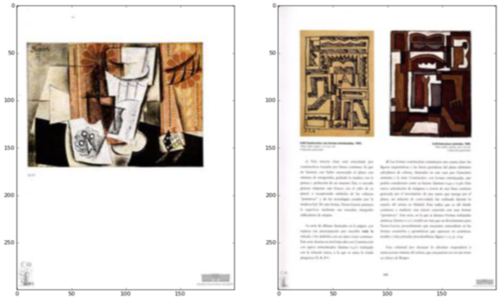
\includegraphics[width=0.8\textwidth]{Figures/similitud_3.png}
\caption{Par de imágenes similares 3}
\end{figure}

\begin{figure}[H]
\centering
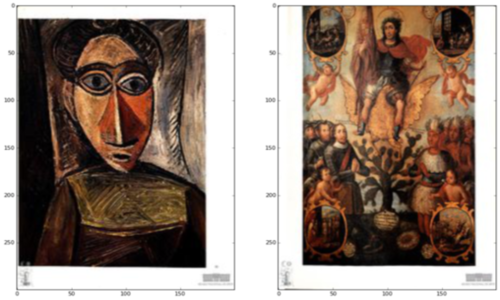
\includegraphics[width=0.8\textwidth]{Figures/similitud_4.png}
\caption{Par de imágenes similares 4}
\end{figure}

\begin{figure}[H]
\centering
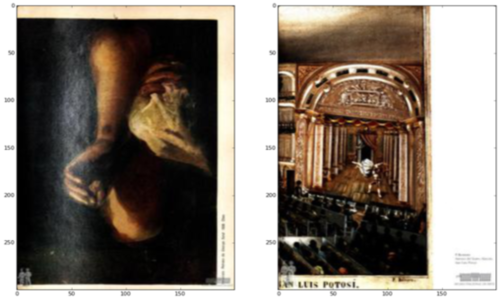
\includegraphics[width=0.8\textwidth]{Figures/similitud_5.png}
\caption{Par de imágenes similares 5}
\end{figure}

Para encontrar la similitud de imágenes se puede realizar una clasificación previa de las mismas, para poder agrupar aquellas imágenes que tienen una estructura de página similar. Es decir, aquellas páginas que tienen imágenes pequeñas dentro de ellas se distingan o se encuentren en un folder diferente de aquellas que tienen imágenes casi del tamaño de la página. Para realizar este proceso de agrupación se utilizaron k-medias, el cual busca agrupar aquellas observaciones que se encuentren más cercanas, siendo la medida de distancia la euclidiana.  Para realizar este proceso, cada imagen se debe convertir a una escala de grises, la matriz de la imagen que da como resultado es convertida en un vector que, dado la transformación previa a 200 x 300, tiene una longitud de 60,000. 

Esta matriz es la necesaria para ejecutar el algoritmo de k-medias, sin embargo, dado la longitud de los vectores y al gran número de páginas sobre las que tiene que calcular distancias, puede llegar a ser muy tardado este proceso, por lo que se decidió que para acelerar este proceso se podía hacer una reducción de dimensionalidad, que permitiera tener un menor número de variables sobre las cuales calcular las distancias. Para ello, se utilizó una descomposición de matrices llamada Singular Value Decomposition, SVD, quedándonos solo con las 8 componentes que capturaron en las pruebas el 40\% de la variabilidad de la matriz (ver \cite{leskovec2014mining}).


Ya con la reducción de las columnas de la matriz, es más rápido hacer el proceso de k-medias y se pueden crear el número de clusters que se desee. Los resultados pueden verse en las figuras \ref{fig:cluster2} y \ref{fig:cluster2}, que son imágenes que pertenecen a los clusters 1 y 2, respectivamente.

\begin{figure}[H]
\centering
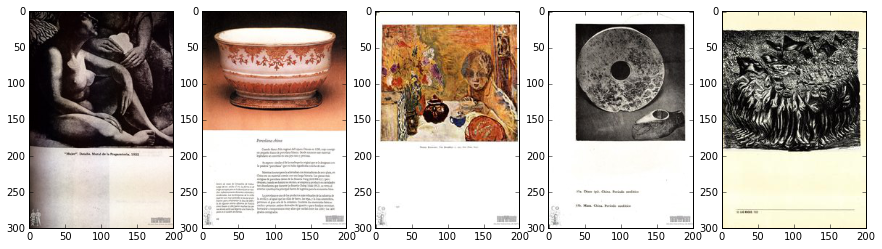
\includegraphics[width=1\textwidth]{Figures/cluster_1.png}
\caption{Muestra 1 de imágenes del cluster 1.}
\label{fig:cluster1}
\end{figure}

\begin{figure}[H]
\centering
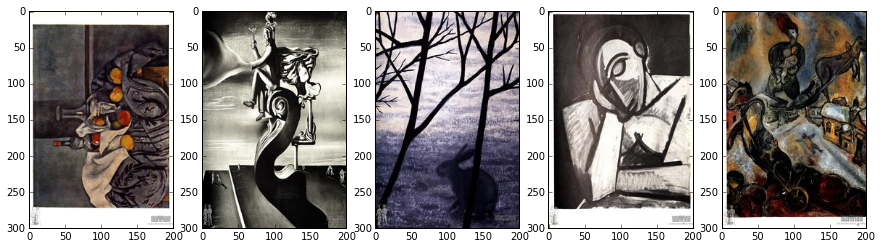
\includegraphics[width=1\textwidth]{Figures/cluster_2.png}
\caption{Muestra 2 de imágenes del cluster 1.}
\label{fig:cluster2}
\end{figure}

Este proceso de agrupación es opcional, y bien puede realizarse antes de correr el algoritmo de Local Sensitive Hashing para realizar similitud sólo sobre páginas con estructura de páginas similares, o bien puede dejarse de lado y correr sobre todas las páginas. Más detalles sobre estos algoritmos los veremos en las secciones siguientes.

\subsection{Filtro de extracción de imágenes}

La primera parte del pipeline consiste en crear un método para identificar las páginas que contienen imágenes, para ello se ha decidido transformar la imagen de color a escala de grises hacer un filtro de varianza. La idea consiste en que aquellas páginas que tienen sólo letras o están vacías tienden a ser más homogéneas, pero aquellas páginas con imágenes son más heterogéneas.





\subsection{ Singular Value Decomposition (SVD) \& K-Means}

Después de identificar para cada libro las páginas que tienen imágenes, copiamos dichos jpgs a una carpeta nueva y reducimos el tamaño del jpg a una estructura de 200 x 300 píxeles. Esto porque al momento de volver la imagen en vector, cada imagen puede tener un diferente número de píxeles oscilando entre los 2000 y los 2500 de ancho y entre 3000 y 3500 de alto, lo que imposibilitaría poder formar una matriz con todas las imágenes. Aunado a lo anterior, una matriz con un ancho de 2500 x 3500 , es decir una matriz con cerca de 8,750,000 columnas, sería intratable. 
Una técnica usual que se puede utilizar para este tipo de problemas
es la descomposición en valores singulares. En este caso, buscamos descomponer
una matriz $X$ de tamaño $nxm$ mediante


$$X=UDV^t$$

donde $U$ y $V$ son matrices ortogonales de tamaño $nxn$, $mxm$ y $D$ es una matriz
rectangular diagonal no negativa de tamaño $nxm$, con los componentes de su diagonal ordenados de forma decreciente (ver \cite{leskovec2014mining}). 

Resulta ser que esta descomposición siempre existe. Ahora supongamos que escogemos una $k$ chica, y definimos
- $U_k$ como la sub-matriz $nxk$  de $U$ donde seleccionamos las primeras $k$ columnas,
-  $V_k$ la sub-matriz $mxk$ de $V$ donde seleccionamos las primeras $k$ columnas,
- $D_k$ una matriz diagonal de $kxk$ (primeros $k$ renglones y $k$ columnas de $D$)

Entonces $X^k=U_k D_k V_k^t$ es \textbf{la matriz de rango} $k$ que minimiza
$$\sum (X_{ij} -X_{ij}^k )^2$$


Desde este punto de vista, esta descomposición parece resolver precisamente el
problema que queríamos: aproximar lo más cercano posible con una descomposición de matrices de rango bajo. En nuestro caso, podríamos tomar

\begin{itemize}
\item $U' = U_k D_k^{1/2}$
\item $V' = D_k^{1/2} V_k$
\end{itemize}

para obtener la descomposición que propusimos arriba. Con la transformación, nos quedaría una matriz con 6,000 columnas y filas como pinturas se encontraran en los libros.


En la colección de documentos hemos encontrado que las imágenes pueden venir de las siguientes maneras : 

\begin{itemize}
\item una imagen por página,
\item varias imágenes por página, 
\item mezcla de páginas y texto
\end{itemize}
Por el momento nos vamos a enfocar en las páginas que sólo tienen una imagen, para ello se realiza  un clustering, que nos sirva para formar grupos de páginas de acuerdo a la estructura. En clustering (o análisis de conglomerados) se busca agrupar “puntos” en “grupos”, de manera que puntos dentro de un cluster estén cercanos entre ellos, mientras que puntos en distintos clusters están a distancia más grande - todo esto de acuerdo a alguna medida de distancia.

K-medas es posiblemente el algoritmo más popular de segmentación, y  escala razonablemente bien a problemas medianos-grandes.

En k\-medias, un buen agrupamiento es uno en el que la variación dentro de los grupos
es chica. En primer lugar fijamos el número $K$ de grupos que buscamos. Supongamos entonces que $C_1\cup\cdots\cup C_K$ es una partición de los
datos, y sea $W(C_k)$ nuestra medida de variación dentro de los clusters. Entonces
buscaremos resolver

$$min_{C_1,\ldots, C_K} \sum_{k=1}^K W(C_k)$$ 

En general, este problema es imposible de resolver por enumeración, pues aún para un conjunto de datos chico con $K$ chica, el espacio de posibles particiones es inmenso.

Sin embargo, escogiendo mediadas $W$ particulares es posible construir algoritmos con desempeño razonable. En primer lugar, suponemos que $W(C)$ está dado por

$$W(C_k) =\frac{1}{|C_k|}\sum_{i,j\in C_k} ||x_i-x_j||^2,$$

es decir, la medida de variación dentro de los clusters es el promedio de distancias
euclídeas al cuadrado dentro del cluster. El problema

$$min_{C_1,\ldots, C_K} \sum_{k=1}^K \frac{1}{|C_k|}\sum_{i,j\in C_k} ||x_i-x_j||^2$$ 

todavía es demasiado difícil. Sin embargo, no es difícil demostrar (usando pitágoras) que

$$W(C_k)=2\sum_{i\in C_k} ||x_i-\bar{x}_k||^2,$$

donde $\bar{x}_k=\frac{1}{|C_k|}\sum_{i\in C_k} x_i$ es el centroide del grupo $C_k$.


y ahora notamos que si los $C_1,\ldots C_K$ están dados, entonces
tenemos que
$$\bar{x}_k = argmin_{m} \sum_{i\in C_k} ||x_i-m||^2,$$

(pues tenemos el teorema: el centroide es el punto con distancia euclidiana cuadrada promedio más baja a los elementos del grupo). Podemos entonces cambiar nuestro
problema original por el problema ampliado

$$min_{C_1,\ldots, C_K, m_1,\ldots, m_k} \sum_{k=1}^K \sum_{i\in C_k} ||x_i-m_k||^2$$ 

Vemos entonces que
\begin{enumerate}

\item  Si tenemos la asignación $C_1,\ldots C_K$, entonces podemos
encontrar las $m_1,\ldots, m_k$ calculando los centroides $m_k = \bar{x}_k$.
\item  Si tenemos los centroides $m_k$ fijos podemos resolver
$$min_{C_1,\ldots C_K} \sum_k \sum_{i\in C_j} ||x_i - m_k||^2$$
asignando cada punto a la $m_k$ más cercana.

\end{enumerate}

El primer paso es crear una matriz  con cada imagen en blanco y negro, en donde cada fila es una página con varianza alta y cada columna el deshilado de la matriz de la imagen en escala de grises, luego utilizaremos la descomposición de valores singulares para reducir la dimensionalidad y para posteriormente utilizar un  clustering con Kmeans. El número de Kmeans lo queremos pequeño pero suficientemente grande para separar bien las páginas, en las pruebas realizada un clustering con k=5 ha tenido un buen desempeño. A continuación se muestran los resultados. 


\subsection{ Local Sensitive Hashing (LSH)}

Para encontrar elementos similares en conjuntos de datos se necesita construir una medida de similitud adecuada, hacer eficiente éste cálculo y definir las reglas para encontrar grupos de objetos de similitud alta. A pesar de ser una técnica de minería de textos aplicamos este concepto para encontrar grupo de imágenes similares. 

Local Sensitive Hashing se concentra solamente en pares de documentos( en este caso imágenes) con alta probabilidad de ser similares ya que calcular todos los pares de similitud es poco factible. La idea central es  encontrar una manera de asignar las imágenes a una colección de cubetas de forma que imágenes con alta similitud caen en la misma cubeta. En este sentido \textbf{LSH} es una especie de clustering de datos (ver \cite{leskovec2014mining}).

En nuestro caso, la salida de LSH es una lista de pares de imágenes con alta
probabilidad de tener similitud alta.


Supongamos que tenemos un total de $k=br$ firmas de minhash\footnote{ minhashing es la reducción de dimensionalidad para estimar eficientemente similitud entre imágenes.} para una colección de imágenes.
Dividimos estas firmas en $b$ bandas (grupos) de $r$ minhashes cada una.

Observamos entonces que

- La probabilidad de que el minhash de una firma en particular coincida para un par de
documentos es $s$, que es el índice de jaccard entre los documentos. \footnote{El índice de jaccard es un estadístico para comparar la similitud de elementos, es definida como la intersección de los dos elementos dividida entre la unión (ver \cite{leskovec2014mining})}

- La probabilidad de que $r$ minhashes de una banda coincidan todos es $s^r$, pues las
funciones hash se seleccionan independientemente.
- La probabilidad de que al menos una de las bandas coincida totalmente es entonces
$1-(1-s^r)^b$ 

En consecuencia, la probabilidad de que al menos coincida una banda de minhashes en
función de la similitud se ve como sigue:

\begin{itemize}

\item Nótese que la probabilidad es 1/2 cuando $s=(1-0.5^{1/b})^{1/r}$
- La probabilidad es mayor a 0.90 cuando $s >(1-0.10^{(1/b)})^{1/r}$
\item Podemos entonces escoger $b$ y $t$ para capturar con alta probabilidad los niveles
de similitud que nos interesen, capturando tan pocos falsos negativos como deseemos.

\end{itemize}


Por ejemplo, si tenemos 20 bandas de tamaño 10, la probabilidad de coincidencia de al menos una banda es mayor a 0.90 cuando $s$ es más grande que 0.92

Una vez que tenemos nuestra matriz, donde cada imagen es una fila y en cada columna tenemos el conteo para cada uno de los colores, usamos Local Sensitive Hashing para determinar las imágenes que eran más similares de acuerdo a sus vectores de colores. Usamos 300 funciones hash, que simplemente son 300 vectores aleatorios de longitud 1,331, y agrupamos en 15 bandas de 20 hashes cada una. Luego del proceso de dividir las imágenes en distintas cubetas, de acuerdo a su similitud, calculamos la distancia coseno entre cada par que estuviera en la misma cubeta.


\section{Conclusión}

El proceso implementado en este trabajo tuvo como finalidad desarrollar una metodología que permitiera identificar imágenes dentro de las páginas y encontrar otras imágenes que fueran parecidas. Para ello se realizaron  4 procesos principales: 

\begin{enumerate}
\item Transformar los colores de cada página a una colección definida de colores.
\item Identificar si la imagen es a colores.
\item Una reducción de las imágenes identificadas. 
\item Construcción de una matriz de conteo de colores.
\item Encontrar similitud de imágenes.
\end{enumerate}

Esta descomposición del trabajo, no solo facilitó el abordar el problema sino que además permitió también programarlo de manera más sencilla en el esquema de \texttt{luigi}, lo que permitió realizar varios de estos procesos en paralelo y así reducir el tiempo de ejecución del proceso total.

La similitud que se encuentre en las imágenes sugeridas debe medirse en razón de los colores y no de los temas o formas tratadas en la pintura. No obstante lo anterior, creemos que esta similitud no es poca cosa ya que gran parte de las emociones que se transmiten en una pintura se debe a la combinación de colores que se emplearon.

\section{Problemas}

 En cada proceso se mencionó si existieron problemas. El principal problema  fue la dificultad 
 para procesar archivos pesados y  encontrar una forma de distinguir las páginas de colores de las que no. 
 
 A pesar de contar con una técnica robusta para distinguir  las páginas con imágenes no se pudo identificar el número de imágenes por página. Esto es relevante porque al momento de hacer conteo de colores, en páginas donde existen dos o más pinturas, se estaría  tomando el conteo de dos imágenes distintas para hacer su vector y al sugerir una imagen parecida se sugeriría  una imagen que se pareciera a la combinación de dos imágenes.

\section{Trabajo futuro}

Una forma de ampliar los resultados desarrollados en el presente trabajo, sería el poder contar con información acerca de las pinturas analizadas, información acerca de los autores, las fechas en las que se realzaron o los países en las que fueron pintadas. Esta información muchas veces se encuentra al pie de las pinturas y obtener esta información sería mucho más fácil si de entrada se supiera que en esa página existe una pintura.

Además, esta información permitiría hacer un análisis mucho más enriquecedor acerca de los colores en la pintura, permitiendo saber qué colores fueron los más utilizados en cada época o por cada autor.

	 
\chapter{Procesamiento de Clickstream}
\label{logs}


\section{Introducción}

En un sitio Web, el análisis de \emph{``clickstream''} es el proceso de
recolección, análisis y presentación de datos agregados sobre cada paso
que siguen los visitantes en una página web y en qué orden, es decir,
son el resultado de la sucesión de clicks del ratón por cada visitante.
Regularmente, dicho flujo o registro de información es almacenado en un
principio para la gestión de los registros y posteriormente son
analizados para producir estadísticas que resulten de utilidad \citep{lagus2000text}.

%\section{ El problema por resolver}\label{el-problema-por-resolver}

En el caso de la biblioteca de arte, los registros de cada click que realizan los usuario en la página de DSpace son almacenados en un archivo común o estándar llamado  \href{https://httpd.apache.org/docs/2.2/logs.html}{access.logs}; estos archivos después de ser estructurados, tienen las principales ventajas de poder conocer a los usuarios y entender sus necesidades de búsqueda, conocer el día a día de las operaciones y en una segunda etapa poder realizar recomendaciones a los usuarios\citep{banerjee2002characterizing}.

Para realizar dicho análisis es necesario obtener y estudiar los datos provenientes de los access log\citep{apache} principalmente porque son datos no estructurados. Una vez estructurados, se necesitan quitar los registros duplicados, sesionizar los datos y enriquecer los registros ya que debido a las características que aporta cada registro, suelen no ser suficientes para tener un análisis más detallado.

Cabe destacar que no sólo la resolución del problema llega hasta esta fase, sino hasta la creación de un dashboard o tablero de estadísticas que ayudan a visualizar las principales características de los datos; por ejemplo, los usuarios que tienen más visitas, su tiempo de permanencia, las páginas más visitadas, entre otras.


\section{Orquestación}\label{orquestacion}

La orquestación se realiza por medio de \href{http://luigi.readthedocs.org/en/stable/}{luigi}, pero para el análisis de \emph{clickstream},  las ventajas que se utilizan son las de \emph{modularidad}, \emph{robustez} e \emph{idempotencia}. Cabe resaltar que para esta fase del proyecto, debido a que no se tienen archivos access log provenientes de \emph{D-space}, los archivos logs fueron obtenidos de diversas fuentes \citep{veterina}; sin embargo, la estructura típica de los access log es la misma para este tipo de archivos.
A continuación se describe los pasos del \emph{pipeline} que son ejecutados por la función principal \emph{analisis-log-itam.py}; en cada uno de estos se explica su función, así como también el archivo \emph{input} y \emph{output} necesario.


\subsubsection{ Inputlog}\label{i-inputlog}

Es el primer paso del pipeline y es el encargado de importar el archivo
\emph{access.logs} de la ruta predeterminada hacia el orquestador
(\emph{luigi}).

Como antecedente, este proceso se ejecutaba por medio de \emph{batch} en
el lenguaje de programación \emph{pearl} por medio de la función
\emph{accesslog2csv.pl}; sin embargo, se decidió integrar este paso a la
orquestación de \emph{luigi} para que el proceso se ejecutado en una
sola orquestación.


\begin{itemize}
\item \textbf{Input}: access.log
\item \textbf{Output}: inputlog.pd (archivo data frame pandas)
\end{itemize}




\subsubsection{ Parsear}\label{ii-parsear}

Después de que \emph{luigi} recibe el access.log,este paso es el
encargado de nombrar las variables y la estructura del archivo
\emph{access.log}. La estructura y los nombres de las variables fueron
tomadas de los \emph{CustomLog}
\href{https://httpd.apache.org/docs/2.2/logs.html}{apache.org}.

Las variables que se tienen son las siguientes:

\begin{itemize}
\itemsep1pt\parskip0pt\parsep0pt
\item
  Host: La dirección IP del usuario que accede al servidor web. \emph{127.0.0.1}
\item
  Log\_Name: El identificador de usuario en la máquina cliente \emph{frank}
\item
  Date\_Time
\item
  Method: Petición enviada por el cliente, inidicando el tipo (normalmente \emph{GET} o \emph{POST}).
\item
  Response\_Code: Código de respuesta de la página \emph{200}
\item
  Bytes\_Sent Es el número de bytes entregados por el servidor en la página de respuesta a la petición.
\item
  URL Es la página en donde se encuentra el enlace que ha generado la petición al servidor
\item
  User\_Agent: Es una cadena que identifica al navegador desde el cual se ha realizado la petición. 
\end{itemize}


\begin{itemize}
\item \textbf{Input}: inputlog.pd
\item \textbf{Output}: parsear.pd
\end{itemize}


\subsubsection{ Usuario}\label{iii-usuario}

En este paso se necesita tener identificados a los usuarios en sentido en la forma en que visitaran la página de DSpace ya que es el servicio de consulta de la biblioteca de arte, puede llevarse a cabo por medio de una computadora por usuario o varios usuarios en una misma computadora. La mejor práctica para identificar a los usuarios en este tipo de páginas, se realiza por medio de tablas intermedias como tablas de acceso, tablas de usuarios y tablas bitácora\citep{andersen2000analyzing}.

En caso de no existir este tipo de tablas intermedias, se tiene que trabajar por medio de suposiciones de como el usuario accede a la página, comúnmente se supone que cada usuario proviene de una IP única, si este no es el caso, se puede hacer el supuesto por medio de IP + buscador que utiliza y así sucesivamente; inclusive se puede hacer de forma heurística tomando en cuenta el tiempo entre páginas.

Para poder realizar este paso, nos basamos en el supuesto que un usuario, solo visitará el sitio por medio de una computadora o IP fija.

\begin{itemize}
\item \textbf{Input}: parsear.pd
\item \textbf{Output}: usuario.pd
\end{itemize}


Este paso es posible que sea modificado ya definida la estructura de
consulta de \emph{D-space}. Dentro de la función
\emph{analisis-log-itam.py} se tiene comentado en dónde se realizaría
dicho cambio.

\subsubsection{ Sesionizar}\label{iv-sesionizar}

La función de este paso es ordenar los registros por fecha y usuario,
quitar duplicados y agregar 2 campos nuevos que son:

\begin{itemize}
\item
  time\_diff: calcula la diferencia en tiempo entre una consultas del
  usuario en la página \emph{web} siendo el primer registro puesto como
  \emph{0} ya que no se tiene contra quien comparar.
\item
  Rank: crea un ``ranking'' entre las consultas por usuario, siendo
  \emph{1} la primera consulta del usuario, \emph{2} la segunda y así
  sucesivamente.
\end{itemize}

Para ejemplificar este paso, se tiene la siguiente tabla

\begin{table}[H]
\centering
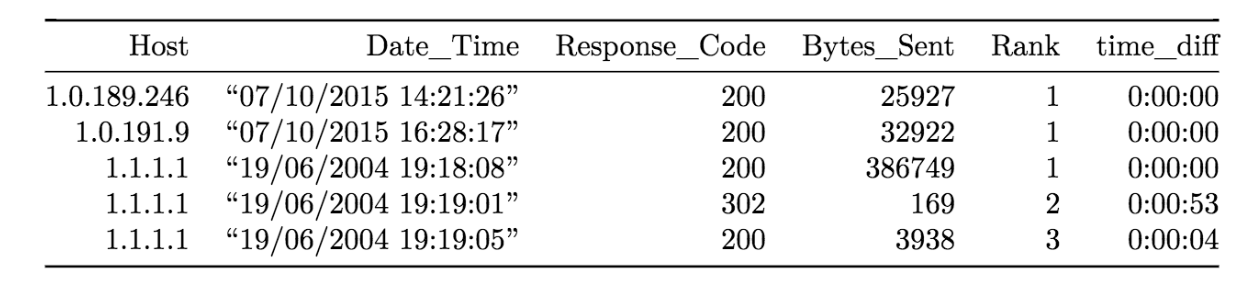
\includegraphics[width=0.8\textwidth]{Figures/tabla1.png}
\caption{Sesionizar}
\end{table}

Se observa que para el primer y segundo dato, sólo existe un registro de acceso en ese día, por lo que su $rank=1$ y su $time\_diff=0$; a partir del tercer datos, se observa que es un usuario con 3 registros, el rank es una secuencia de 1 a 3 en orden del tiempo y el campo de time diff siempre será 0 en el $rank=1$ y posteriormente realizará la diferencia entre registros.

\begin{itemize}
\item \textbf{Input}: usuario.pd
\item \textbf{Output}: sesionizar.pd
\end{itemize}



\subsubsection{Enriquecer}\label{v-enriquecer}

En este paso se crean nuevas variables o campos que podrían ser de
interés para el análisis. Los campos que se crean por consulta son los
siguientes:

\begin{itemize}
\itemsep1pt\parskip0pt\parsep0pt
\item
  year: año
\item
  month: mes
\item
  day: dia (número)
\item
  hour: hora
\item
  day of week: día de la semana
\item
  dif seg clicks: segundos de consulta
\end{itemize}

En este paso, pueden ser agregados más campos que sean de interés para
los administradores del sistema. Los campos descritos con anterioridad
son los más comunes ya que nos ayudan a determinar los días, horas, mes
y años de visitas más o menos frecuentes y/o el tiempo promedio de permanencia.

Un ejemplo de este paso sería el siguiente

\begin{table}[H]
\centering
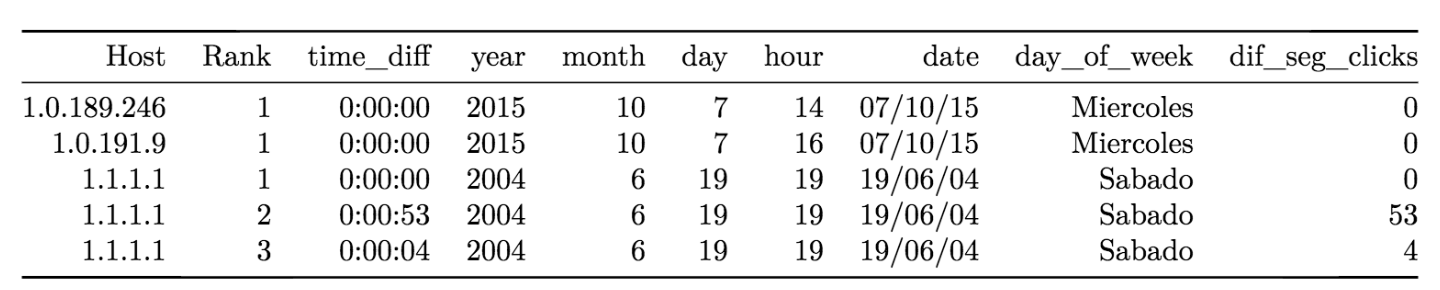
\includegraphics[width=1\textwidth]{Figures/tabla2.png}
\caption{Enriquecer}
\end{table}

El cual simplemente agrega campos que podrían ser de interés para el usuario. El output es de tipo \emph{csv} y es el insumo principal del dashboard.

\begin{itemize}
\item \textbf{Input}: sesionizar.pd 
\item \textbf{Output}: enriquecer.csv o enriquecer.pd
\end{itemize}


\subsubsection{ Reportes}\label{vi-reportes}

De manera automática son creados reportes en \emph{pdf} de los
\emph{códigos de respuesta} y \emph{usuarios} con las estadísticas del
porcentaje de visitas y el tiempo promedio de consulta.

\begin{itemize}
\item \textbf{Input}: enriquecer.pd
\item \textbf{Output}: reportes.pdf
\end{itemize}


\begin{figure}[H]
\centering
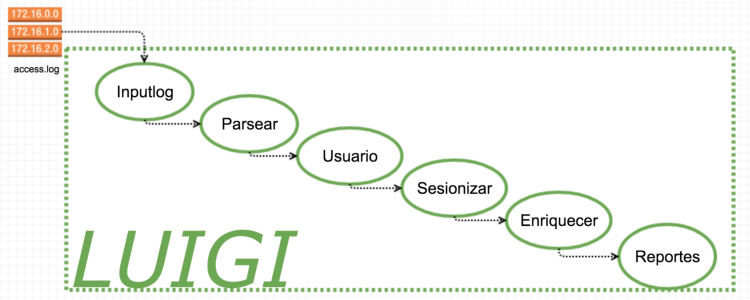
\includegraphics[width=1\textwidth]{Figures/unnamed-chunk-1-1}
\caption{Pipeline del análisis de clickstream}
\end{figure}

\section{Conclusión}

 Con lo investigado dentro de este capítulo, se ha demostrado que el análisis de clickstream es necesario realizarlo con la información generada por el Dspace, ya que como se tiene la completa administración del portal, por medio de los access log, se pueden llevar a cabo un conocimiento profundo de los usuarios con la finalidad de entender sus necesidades de búsqueda y conocer el día a día de sus actividades ya que al tener este tipo de información, se pueden crear recomendaciones para los usuarios recurrentes y los nuevos usuarios. A su vez, también este tipo de análisis ayuda de manera interna (en cuanto a administración), de como está operando el portal ya que es posible detectar posibles problemas por medio de los códigos de respuesta.


\section{Problemas}\label{Problemas que pueden surgir}

Existen 2 tipos principales de archivos logs que son de accesos y error, y dentro de estos se encuentran a su vez otros tipos de archivos; 
por ejemplo, para el caso del tipo access log se encuentran CustomLog (que son los utilizados en el presente estudio), LogFormat y SetEnvIf.
Como la categoría principal es la de access CustomLog, los problemas radican cuando se piensa que se tiene un CustomLog y en realidad es otro tipo de archivo, por lo que al realizar el paso que estructura los datos, el formato es distinto y se tenga un error en cuanto a estructura.

Otro problema está en el paso de detección de usuarios, un mismo usuario puede acceder a un determinado portal desde diferentes computadoras, por ejemplo, desde su casa o la oficina; esto no implica que el análisis de los logs, sean inútiles, pero su funcionamiento está diseñado cuando se identifican a usuarios  registrados o se les realiza alguna recomendación.



\section{Trabajo futuro}\label{trabajo futuro}

Las líneas futuras de investigación existentes que pueden contemplar el análisis, son muchas; sin embargo, se puntualizaran las necesarias a realizar en un futuro cercano:

\begin{itemize}
\item Crear un modelo de recomendaciones a los usuarios basados en filtros colaborativos
\item Tener un seguimiento del éxito de las recomendaciones
\item Identificación de nuevos usuarios para asignar recomendación con base en los usuarios ya existentes.
\item Medición de los códigos de respuesta para conocer posibles errores internos del portal.
\end{itemize}

	\chapter{Instalación}
\label{ch:guia}


La instalación puede parecer un poco repetitiva pero la idea es que cada parte del producto final se ejecute en un Docker independiente (ver detalles más adelante), así que, en esta sección se pretende explicar los requerimientos necesarios para cada una de las partes y después hacer una breve guía de uso de las mismas.

\section{Instalación procesamiento de texto}

La instalación del paquete para el procesamiento de texto en Ubuntu es bastante simple. Se requiere instalar \texttt{Python}, \texttt{R} y algunas pocas librerías de \texttt{Python} usando \texttt{apt-get} y las demás se instalan solas al instalar la librería \texttt{itm}. Cabe mencionar que el proceso puede correr incluso si no están instaladas correctamente todas las dependencias, pero los procesos que las utilicen fallarán.

\begin{lstlisting}
 
# Necesario para instalar R >= 3.1
echo "deb http://cran.rstudio.com/bin/linux/ubuntu trusty/" >> /etc/apt/sources.list && \
	sudo apt-key adv --keyserver keyserver.ubuntu.com --recv-keys E084DAB9

# Actualizar indices de apt-get
sudo apt-get update && \
	apt-get upgrade # Necesario para instalar R >= 3.1

# Instalar Python	2.7 y PyPi
sudo apt-get install -y \
	python2.7-dev \
	python-pip

# Instalar R (debe ser >= 3.1)
sudo apt-get install -y \
	r-base \
	r-base-dev && \
	R --version

# Librerias de algebra lineal, Fortran y compilador de Markdown
sudo apt-get install -y \
	libblas-dev \
	liblapack-dev \
	gfortran \
	pandoc

# Instalar el paquete itm	y sus dependencias de Python
PACK = /ruta/a/paquete/itm-a.b # Donde a.b es la versi\'on (ej: itm-0.3)
pip install $PACK

# Instalar librerias de R y bajar stopwords de nltk (no se bajan al bajar el paquete)
R -e 'install.packages(c("dplyr", "optparse", "networkD3"), repos = "http://cran.us.r-project.org")'
python -c "import nltk; nltk.download('stopwords')"
\end{lstlisting}


\section{Instalación procesamiento de imágenes}

\begin{lstlisting}
#Instalar R

sudo sh -c 'echo "deb http://cran.rstudio.com/bin/linux/ubuntu trusty/" \
>> /etc/apt/sources.list'

gpg --keyserver keyserver.ubuntu.com --recv-key E084DAB9
gpg -a --export E084DAB9 | sudo apt-key add -

sudo apt-get update
sudo apt-get -y install r-base

#Instalar paquetes
sudo su - -c "R -e \"install.packages('dplyr', \
repos='http://cran.rstudio.com/', dependencies = TRUE)\""
sudo su - -c "R -e \"install.packages('jpeg',\
repos='http://cran.rstudio.com/', dependencies = TRUE)\""
sudo su - -c "R -e \"install.packages('lsa', \
repos='http://cran.rstudio.com/')\""

##Instalar paquetes python

sudo apt-get install python-numpy python-scipy \
python-matplotlib ipython ipython-notebook \
python-pandas python-sympy python-nose \
python-skimage

sudo apt-get install python-pip
sudo pip install -U scikit-learn


#Instalar luigi

wget https://pypi.python.org/packages/source/l/luigi/luigi-2.0.0.tar.gz#md5=06258afcfcdd2f829167450fd5fed604
tar -xzvf luigi-2.0.0.tar.gz
cd luigi-2.0.0/
sudo python setup.py install

#instalar imagemagick
sudo apt-get install imagemagick

##Instalar tornado para que funcione el central scheduler
wget https://pypi.python.org/packages/source/t/tornado/tornado-4.3.tar.gz
tar -xzvf tornado-4.3.tar.gz
cd tornado-4.3
python setup.py install

##Copio los scripts a mi instancia
scp -r Luigi_Imagenes root@ip_instancia:/home
\end{lstlisting}

\section{Instalación para el análisis de logs}

Para la ejecución del pipeline de análisis de Logs es necesario instalar \texttt{Python}, \texttt{R} y bibliotecas de \texttt{Python} usando \texttt{apt-get}


\begin{lstlisting}
# Necesario para instalar R >= 3.1
echo "deb http://cran.rstudio.com/bin/linux/ubuntu trusty/" >> /etc/apt/sources.list && \
	sudo apt-key adv --keyserver keyserver.ubuntu.com --recv-keys E084DAB9

# Actualizar indices de apt-get
sudo apt-get update && \
	apt-get upgrade # Necesario para instalar R >= 3.1

# Instalar R (debe ser >= 3.1)
sudo apt-get install -y \
	r-base \
	r-base-dev && \
	
# Instalar dependencias de R
R -e 'install.packages(c("dplyr", "shiny", "ggplot2"), repos = "http://cran.us.r-project.org")'

# Instalar Python
sudo apt-get install build-essential checkinstall

sudo apt-get install libreadline-gplv2-dev libncursesw5-dev \
libssl-dev libsqlite3-dev tk-dev libgdbm-dev libc6-dev libbz2-dev

sudo apt-get install python2.7

# Instalar dependencias de Python

sudo pip install luigi
sudo apt-get install python-matplotlib
\end{lstlisting}

\section{Instalación Docker}

Para facilitar la instalación anterior se decidió instalar una máquina virtual por medio de Docker, un servicio para administrar Máquinas Virtuales. Docker facilita la instalación y hace la copia de las máquinas un proceso muy simple. El objetivo es poder ejecutar aplicaciones tan complejas como sea necesario en cualquier lugar de una manera sencilla. Los servicios en la nube como Amazon utilizan esta herramienta para poder montar aplicaciones por medio de máquinas virtuales fáciles de preparar.

Para instalar Docker en Ubuntu se siguió las sugerencias de la página \href{http://docs.docker.com/engine/installation/ubuntulinux/}{Instalación Docker}. Es decir, basta con ejecutar los siguientes comandos:

\begin{lstlisting}
# Actualizar apt-get
sudo apt-get update

# Instalar el paquete recomendado
sudo apt-get install linux-image-extra-$(uname -r)

# Instalar Docker
sudo apt-get install docker-engine

# Empezar el servidor
sudo service docker start

# Correr una maquina virtual
# NOTA este comando descarga una imagen con Ubuntu
sudo docker run ubuntu
\end{lstlisting}

Una vez instalado Docker,  se puede descargar la siguiente imagen de una máquina virtual que contiene los paquetes necesarios para ejecutar el procesamiento de imágenes y de texto junto con el análisis de logs.

\begin{lstlisting}
# Descarga la maquina con el procesamiento de texto
sudo docker pull carpetri/itam_tm:v0.3

# Descarga la maquina con el procesamiento de imagenes
sudo docker pull jared275/luigimage
\end{lstlisting}


%FALTA PONER LA MAQUINA DE LOGS

\section{Breve guía de uso}
\subsection{Guía para el procesamiento de texto}

Una vez instalado Docker con  el paquete se puede acceder a los ejecutables desde la consola. Para facilitar su uso se escribieron dos \emph{wrappers}, uno \emph{simple} que sólo pide los parámetros indispensables (\texttt{itam-tm-default}) y otro \emph{avanzado} (\texttt{itam-tm}) que requiere que se especifique todos los parámetros de entrada internos del proceso de \texttt{luigi}. El ejecutable \emph{avanzado} corre un solo proceso a la vez y se debe conocer cómo funciona internamente el paquete, mientras que el \emph{simple} corre todos los análisis para valores especificados de los parámetros.

A continuación se muestra cómo utilizar el \emph{simple} para correr el análisis. Con el fin de probar la instalación y que todo corriera sin problemas, se instaló el paquete en un contenedor de Docker, desde donde se ejecutará todo.

Para empezar hay que ejecutar la máquina virtual que contiene el Docker de procesamiento de texto con el siguiente comando:


 Notar que la bandera \-p es para el puerto. La bandera \-v es para poder ver la carpeta con los libros (en este caso ITAM). Además es importante porque aquí será donde se verán los resultados.
\begin{lstlisting}
sudo docker run -it --name proceso_texto -p 8082:8082 -v /home/dspaceadmin/ITAM/:/home/itam/ carpetri/itam_tm:v0.3 /bin/bash

\end{lstlisting}

Se empieza con una carpeta \texttt{test} en donde están los datos crudos:

\begin{lstlisting}
root@7351c9042a96:/home/itam# ls -lh test
total 0
drwxr-xr-x 1 1000 staff 340 Oct 27 01:49 jpg
drwxr-xr-x 1 1000 staff 340 Nov  3 22:32 pdf
root@7351c9042a96:/home/itam# ls -lh test/pdf/
total 0
drwxr-xr-x 1 1000 staff  748 Oct 27 01:49 1200_years_of_italian_sculpture
drwxr-xr-x 1 1000 staff  680 Oct 27 01:49 12_dibujos_de_jose_maria_velasco
drwxr-xr-x 1 1000 staff 2.8K Oct 27 01:49 20_dibujos_mexicanos_de_maroto
drwxr-xr-x 1 1000 staff 2.5K Oct 27 01:49 revue_des_peintres
drwxr-xr-x 1 1000 staff  952 Oct 27 01:49 tehuantepec
drwxr-xr-x 1 1000 staff 1.8K Oct 27 01:49 vitral
drwxr-xr-x 1 1000 staff  884 Oct 27 01:49 zuniga
drwxr-xr-x 1 1000 staff  918 Oct 27 01:50 zurbaran
root@7351c9042a96:/home/itam# ls -lh test/pdf/zuniga/
total 12M
-rw-r--r-- 1 1000 staff 278K Oct 27 01:49 zun-ctp_00000001.pdf
-rw-r--r-- 1 1000 staff 261K Oct 27 01:49 zun-int_00000001.pdf
-rw-r--r-- 1 1000 staff 168K Oct 27 01:49 zun-int_00000002.pdf
-rw-r--r-- 1 1000 staff 208K Oct 27 01:49 zun-int_00000003.pdf
-rw-r--r-- 1 1000 staff 164K Oct 27 01:49 zun-int_00000004.pdf
-rw-r--r-- 1 1000 staff 139K Oct 27 01:49 zun-int_00000005.pdf
\end{lstlisting}

El siguiente paso es inicializar el servidor de \texttt{luigi}, con el comando siguiente (o alternativamente, se puede agregar \texttt{--local-sceduler} al llamar \texttt{itam-tm-default}):

\begin{lstlisting}
root@7351c9042a96:/home/itam# luigid --background &
\end{lstlisting}

Lo anterior deja el servidor corriendo en segundo plano de manera silenciosa. En la dirección IP `8082` \texttt{luigi} genera un dashboard desde el cual se puede ver el avance. Se puede acceder a él desde un navegador yendo a la dirección \texttt{localhost:8082}. Ya con eso andando sólo es necesario correr el siguiente comando (parámetros de ejemplo):

\begin{lstlisting}
root@7351c9042a96:/home/itam# itam-tm-default \
  -d test \
  --identifier prueba \
  --no-timestamp \
  --languages spanish,english \
  --clean-level clean,stopwords
  --topic-range-lda 3,10,2 \
  --topic-range-lsi 40,81,20 \
  --workers 6
\end{lstlisting}

Los parámetros equivalen a lo siguiente:
\begin{itemize}

\item \texttt{-d, --root-directory [ruta/maestra]} es la ruta que contiene la carpeta \texttt{pdf}.

\item \texttt{--languages idioma1[,idioma2[,...]]} son los idiomas a procesar. Hay que notar que siempre se limpian todos los textos que no hayan sido procesados antes. Esta bandera afecta desde la creación del diccionario y el corpus en adelante.
\item  \texttt{-i, --indentifier [nombre]} le pone el sufijo `nombre` a las carpetas de modelos y resultados con el \item  \texttt{[--no-timestamp]} no poner \textbf{timestamp} en el nombre de las carpetas de modelos y resultados después del identificador.
\item \texttt{[--no-md5]} no revisar las sumas MD5 de los PDFs de entrada ni ponerla en el nombre de las carpetas de modelos y resultados después del \textbf{timestamp} (si hay).
\item \texttt{--clean-level (raw|clean|stopwords)[,(raw|clean|stopwords)[,...]]} agrega los niveles de limpieza a procesar y a modelar.
\item  \texttt{--topic-range-lda start,stop+1,step} hace un modelo LDA para cada nivel de limpieza y para cada número de tópicos, para `start, start + step, ..., stop`.
\item \texttt{--topic-range-lsi start,stop+1,step} hace un modelo LSI para cada nivel de limpieza y para cada número de tópicos, para `start, start + step, ..., stop`.
\item  \texttt{--workers n} lleva a cabo el proceso de extracción y limpieza con \texttt{n} procesos en paralelo.

\end{itemize}

Una vez corriendo lo anterior, el dashboard se ve, por ejemplo, como en la figura (\ref{fig:luigi-dashboard}), qué procesos están corriendo, han sido terminados o faltan por correr. También se puede filtrar los procesos y ver sus árboles de dependencias entre otras cosas.

\begin{figure}[H]
\centering
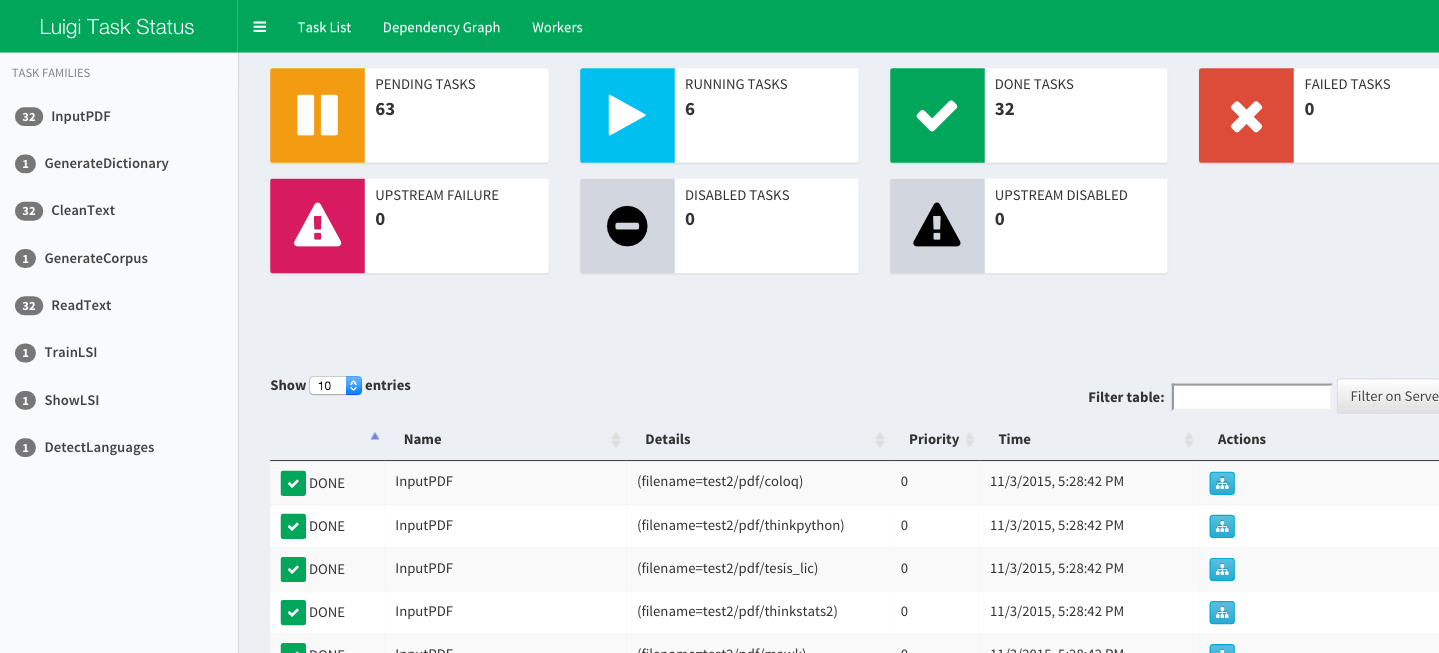
\includegraphics[width=1\textwidth]{Figures/dashboard.png}
\caption{Dashboard de \texttt{luigi} corriendo en el navegador.\label{fig:luigi-dashboard}}
\end{figure}


El dashboard provee muchas formas prácticas para filtrar las tareas, según si están corriendo (azul), si terminaron (verde), si tuvieron algún problema (rojo) o si están pendientes (amarillo). Se puede ver también la información más relevante, como qué proceso está corriendo y con qué parámetros y qué proceso se está encargando de hacerlo. \texttt{Luigi} también proporciona una vista de red, en la que se puede ver gráficamente el árbol de dependencias, como se puede ver en la figura (\ref{fig:lsi-tree}).

\begin{figure}[H]
\centering
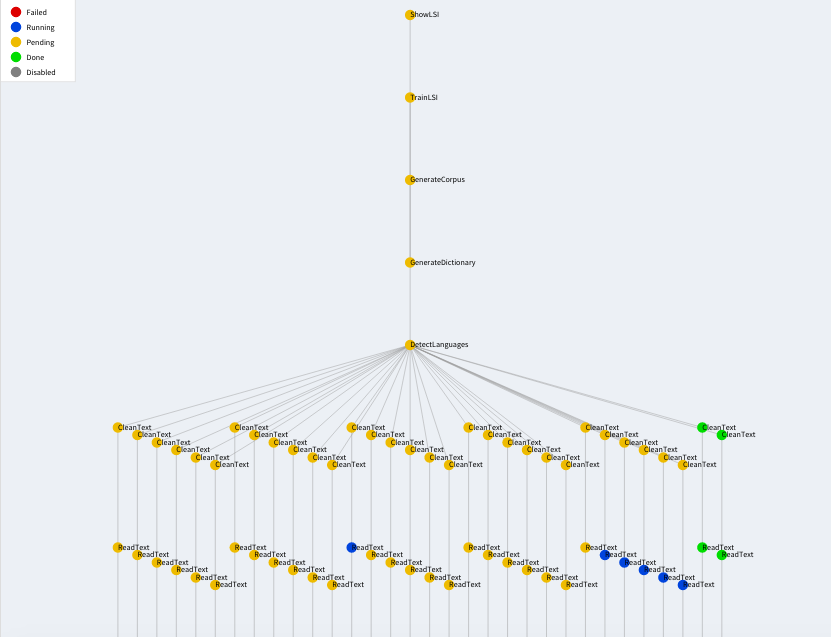
\includegraphics[width=1\textwidth]{Figures/detail.png}
\caption{Árbol de dependencias del LSI con seis procesos corriendo en paralelo.\label{fig:lsi-tree}}
\end{figure}


Con la gráfica es fácil ilustrar algunas de las ventajas del orquestador. Por ejemplo, si se agregan dos libros a la colección, sólo corren los procesos que son estrictamente necesarios (aquí, los modelos, etc.), pero no la limpieza que ya haya sido ejecutada, ya que  \texttt{Luigi} detecta automáticamente qué hay que correr y qué ya no es necesario. En la figura (\ref{fig:luigi-parallel}) se ejemplifica esto.


\begin{figure}[H]
\centering
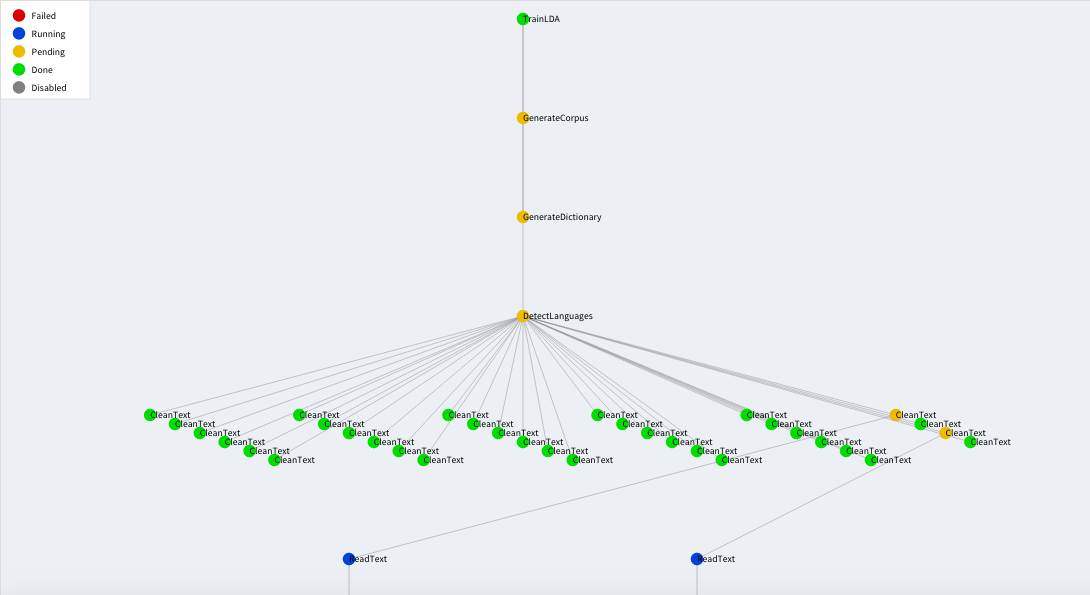
\includegraphics[width=1\textwidth]{Figures/detail2.png}
\caption{Árbol de dependencias del LSI con dos libros que no habían sido procesados.\label{fig:luigi-parallel}}
\end{figure}

\subsection{Guía para  el procesamiento de imagen}

Para empezar hay que ejecutar la máquina virtual que contiene el Docker de procesamiento de imágenes con el siguiente comando:


\# Notar que la bandera \-p es para el puerto. La bandera \-v es para poder ver la carpeta con los libros (en este caso ITAM). Además es importante porque aquí sera donde se verán los resultados.
\begin{lstlisting}
sudo docker run -it --name proceso_imagenes -p 8082:8082 -v /home/dspaceadmin/ITAM/:/home/itam/ jared275/luigimage /bin/bash
\end{lstlisting}

Se decidió realizar pruebas antes de correr el proceso sobre todas las imágenes, por lo que se colectaron 100 libros aleatorios que se guardaron en \texttt{/home/dspaceadmin/ITAM/Libros\_prueba}.

El proceso por el cual se escogieron los 100 libros de manera aleatoria se hizo con el siguiente script:

\begin{lstlisting}
ls /export/librarian | sort --random-sort | head -100 | parallel 'cp -r /export/librarian/{} /home/dspaceadmin/ITAM/Libros_prueba/'
\end{lstlisting}

Con lo anterior ya se puede entrar a la máquina con el procesamiento de imágenes con el comando 

\begin{lstlisting}
sudo docker start -ia proceso_imagen_prueba
\end{lstlisting}

Una vez dentro del Docker se pueden ver  los 100 libros de prueba con la salida:

\begin{lstlisting}
root@18e42a789d4f:/home/itam# ls -la Libros/        
total 408
drwxrwxr-x 102 1000 1000 4096 Nov 21 19:37 .
drwxr-xr-x  16 root root 4096 Dec  2 17:45 ..
drwxrwxr-x   4 1000 1000 4096 Nov 21 19:33 alfredo_zalce_artista
drwxrwxr-x   4 1000 1000 4096 Nov 21 19:31 antonio_ruiz_el_corcito
drwxrwxr-x   4 1000 1000 4096 Nov 21 19:27 biblioteca_de_chapulin
drwxrwxr-x   4 1000 1000 4096 Nov 21 19:30 blanco_y_negro_revista_ilustrada_7_de_abril_de_1918_n._1.403
drwxrwxr-x   4 1000 1000 4096 Nov 21 19:33 calendario_de_galvan_1843
drwxrwxr-x   4 1000 1000 4096 Nov 21 19:31 calendario_de_galvan_pra_el_ano_de_1841
...
\end{lstlisting}

Ahora se está listo para ejecutar el proceso. Para esto los parámetros a elegir son:

\begin{itemize}
\item \texttt{--directorio-libros}: Una liga que apunte al directorio en donde se encuentran los libros con los jpeg.
\item \texttt{--workers} n: lleva acabo el proceso con $n$ procesos en paralelo.
\end{itemize}

Finalmente para ejecutar el proceso basta con escribir el comando a continuación:

\begin{lstlisting}
cd Luigi_Imagenes
python data_flow_EInfo.py LocalSensitiveHashing --directorio-libros \ /home/itam/Libros --workers 12
\end{lstlisting}

Este proceso tardó aproximadamente 3 horas en correr, por lo que se calcula, si se conservan los tiempos vistos en esta prueba, que correrlo sobre los  3,625 libros tardará aproximadamente 110 horas.

El resultado de este pipeline se puede ver el archivo de similitudes

\begin{lstlisting}
root@18e42a789d4f:/home/itam/Luigi_Imagenes# cat 100_libros_similitudes_paginas.csv  | head -7
"","V1","V2","V3"
"","0.93","connecticut_william_hubbellxxYxxcwh-int_00000054.jpg",
"peintres_du_xx_e_sieclexxYxxpein-dxx-int_00000057.jpg"
"","0.98","ritvale_sacri_et_regalisxxYxxrser-int_00000184.jpg",
"ritvale_sacri_et_regalisxxYxxrser-int_00000440.jpg"
"","0.99","ritvale_sacri_et_regalisxxYxxrser-int_00000323.jpg",
"ritvale_sacri_et_regalisxxYxxrser-int_00000325.jpg"
"","0.97","ritvale_sacri_et_regalisxxYxxrser-int_00000106.jpg",
"ritvale_sacri_et_regalisxxYxxrser-int_00000109.jpg"
"","0.83","cezanne_la_obra_de_una_vidaxxYxxczz-int_00000052.jpg"
,"the_art_of_the_printxxYxxtatp-int_00000065.jpg"
"","0.91","alfredo_zalce_artistaxxYxxaza-int_00000056.jpg",
"cezanne_la_obra_de_una_vidaxxYxxczz-int_00000051.jpg"
\end{lstlisting}

\subsection{Guía para el procesamiento de clickstream}\label{instalacion}


\subsubsection{Breve guía de uso}\label{breve-guia-de-uso}

Una vez instalado lo anterior, se necesitan 3 cosas para ejecutar el
pipeline correctamente, la función \emph{analisis-log-itam.py}, el
archivo \emph{access.log} y la carpeta de \emph{functions} la cuál trae
funciones externas. Lo necesario deberá estar en una ruta especificada
por el usuario.

En la línea de comandos ir hasta la ruta donde se tiene lo anterior

\begin{lstlisting}
#Ejemplo:
  cd User/miruta/misarchivos
  
\end{lstlisting}

Para ejecutar el pipeline y visualizar el proceso es necesario abrir
otra línea de comandos y el navegador

\begin{lstlisting}
#Dentro de la linea de comandos teclear:

  luigid

#Dentro del navegador, abrir el puerto y poner la siguiente direccion:

  http://localhost:8082/static/visualiser/index.html#
\end{lstlisting}

Posteriormente en la línea de comandos (diferente a donde se tecleo
\emph{luigid}), ejecutar la función.

\begin{lstlisting}
python analisis-log-itam.py Enriquecer --input-file access.log --output-file\
usuario.pd  --output-df sesionizar.pd --output-df1 enriquecer --output-df2\
reporte.pd
\end{lstlisting}

La salida que se obtendrá será la siguiente

\begin{lstlisting}
===== Luigi Execution Summary =====

Scheduled 5 tasks of which:
* 1 present dependencies were encountered:
    - 1 Inputlog(filename=access.log)
    
* 4 ran successfully:

    - 1 Sesionizar(input_file=access.log, output_file=usuario.pd,
    output_df=sesionizar.pd, output_df1=enriquecer)
    - 1 Parsear(input_file=access.log, output_file=usuario.pd)
    
    - 1 Enriquecer(input_file=access.log, output_file=usuario.pd,
    output_df=sesionizar.pd, output_df1=enriquecer, output_df2=reporte.pd)
    
    - 1 Usuario(input_file=access.log, output_file=usuario.pd, output_df=sesionizar.pd)

This progress looks :) because there were no failed tasks or
missing external dependencies

===== Luigi Execution Summary =====
\end{lstlisting}

Una vez ejecutado, dentro de la ruta se crearan 5 archivos que son los
outputs descritos con anterioridad \emph{reporte.pd},
\emph{sesionizar.pd}, \emph{usuario.pd} y \emph{enriquecer.csv}

Dentro del navegador que se haya abierto con anterioridad se tendrá la siguiente vista:

\begin{figure}[H]
\centering
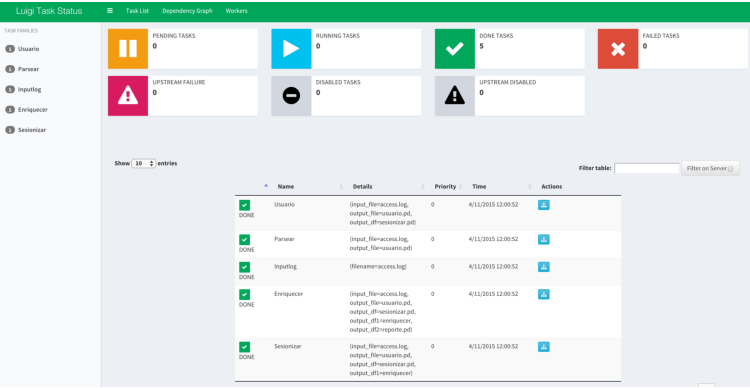
\includegraphics[width=1\textwidth]{Figures/unnamed-chunk-2-1}
\caption{Dashboard de luigi-análisis clickstream}
\end{figure}

\begin{figure}[H]
\centering
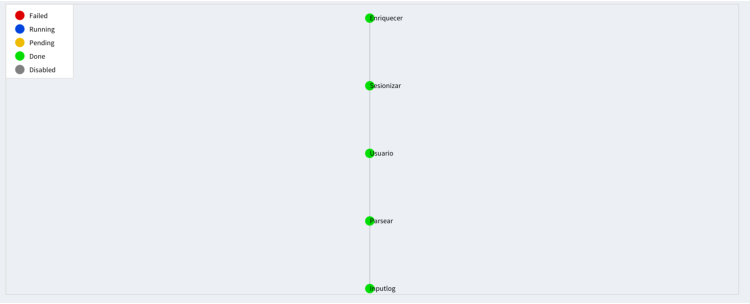
\includegraphics[width=1\textwidth]{Figures/unnamed-chunk-3-1}
\caption{Árbol de dependencias clickstream}
\end{figure}



\subsection{ Ejecución Dashboard}\label{ejecucion-dashboard}

Para poder ejecutar el dashboard es necesario que en la ruta
especificada por el usuario (la cual debe ser la misma donde se
obtuvieron los outputs y el archivo enriquecer.csv), es necesario tener
la carpeta \emph{/R} la cual a su vez tiene dos archivos \emph{server.R}
y \emph{ui.R}

Nuevamente en la línea de comandos, ejecutar:

\begin{lstlisting}
R \-e \textquotedblleft shiny::runApp(\textasciitilde /User/.../R/shinyapp) \textquotedblright
\end{lstlisting}

Al ejecutarse, se tendrá la siguiente salida:

\begin{lstlisting}
> shiny::runApp('~/Desktop/conacyt/R/shinyapp')
Loading required package: shiny
This version of Shiny is designed to work with htmlwidgets >= 0.4. 
Please upgrade your version of htmlwidgets.


Listening on http://127.0.0.1:5127
\end{lstlisting}

El puerto donde se ejecuta el dashboard será el hostname que se muestra,
el cual se tendrá que copiar y pegar en el navegador para poder observar
el dashboard.

Si todo es correcto, se mostrará lo siguiente:

\begin{figure}[H]
\centering
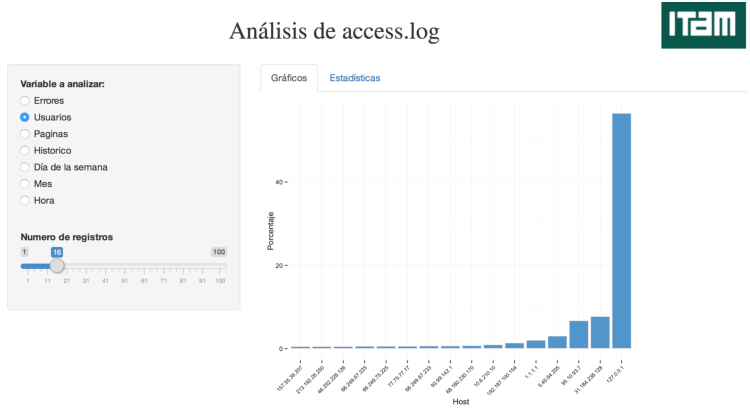
\includegraphics[width=1\textwidth]{Figures/unnamed-chunk-4-1}
\caption{Dashboard  gráficos}
\end{figure}

\begin{figure}[H]
\centering
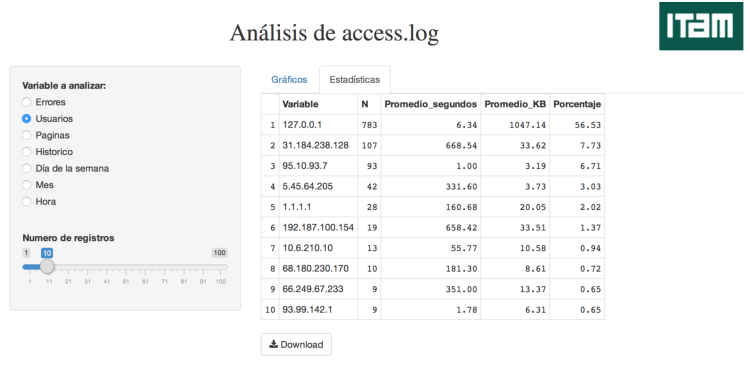
\includegraphics[width=1\textwidth]{Figures/unnamed-chunk-5-1}
\caption{Dashboard  estadísticas}
\end{figure}

En la parte del dashboard, además de poder visualizar las estadísticas
de las variables más importantes, se podrá descargar en formato
\emph{csv} la consulta que le interese al usuario y si esta no le
satisface, podrá descargar los insumos completos.



    %\include{Chapters/trabajo_fut}

    %%%%%%%%%%%%%%%%%%%%%%%%%%%%%%%%%%%%%%%%%%%%%%
	% BIBLIOGRAPHY
	%%%%%%%%%%%%%%%%%%%%%%%%%%%%%%%%%%%%%%%%%%%%%%
	\addcontentsline{toc}{chapter}{Bibliografía} %Añadimos la bibliografia a la lista de contenidos.
	\nocite{*}
	\phantomsection
	\printbibliography

	%%%%%%%%%%%%%%%%%%%%%%%%%%%%%%%%%%%%%%%%%%%%%%
	% APPENDIX
	%%%%%%%%%%%%%%%%%%%%%%%%%%%%%%%%%%%%%%%%%%%%%%
	%\appendix
	%\include{Chapters/appendixA}


%\clearpage
	%


\end{document}

%%% Local Variables:
%%% mode: latex
%%% TeX-master: t
%%% End:
